\chapter{Systematics Uncertainties}\label{sys_uncert}

The systematic uncertainties from different sources are listed in table \ref{tab:SystUncert}.  In this chapter we describe in detail how they were determined for background estimation and signal prediction.

\section{Systematic uncertainties in the background estimation}\label{sys_uncert_bkg}

To estimate the systematic uncertainties for the normalisation of the background prediction we perform a fit in data with different template functions. The figure \ref{fig:fitprunedData} shows the pruned jet mass distribution for different categories and the fits using different models. Base on these fits we can estimate the yields in the signal region and assess a systematic uncertainty ($\delta$) for the background normalisation, as it is shown in Table \ref{tab:backyields2}.  

\begin{figure}[!ht]
\caption{ Fit of the pruned jet mass in data using different template functions in order to estimate an uncertainty for the background normalisation. (left): High purity category (right) : Low purity category.}
\begin{tabular}{cc}
  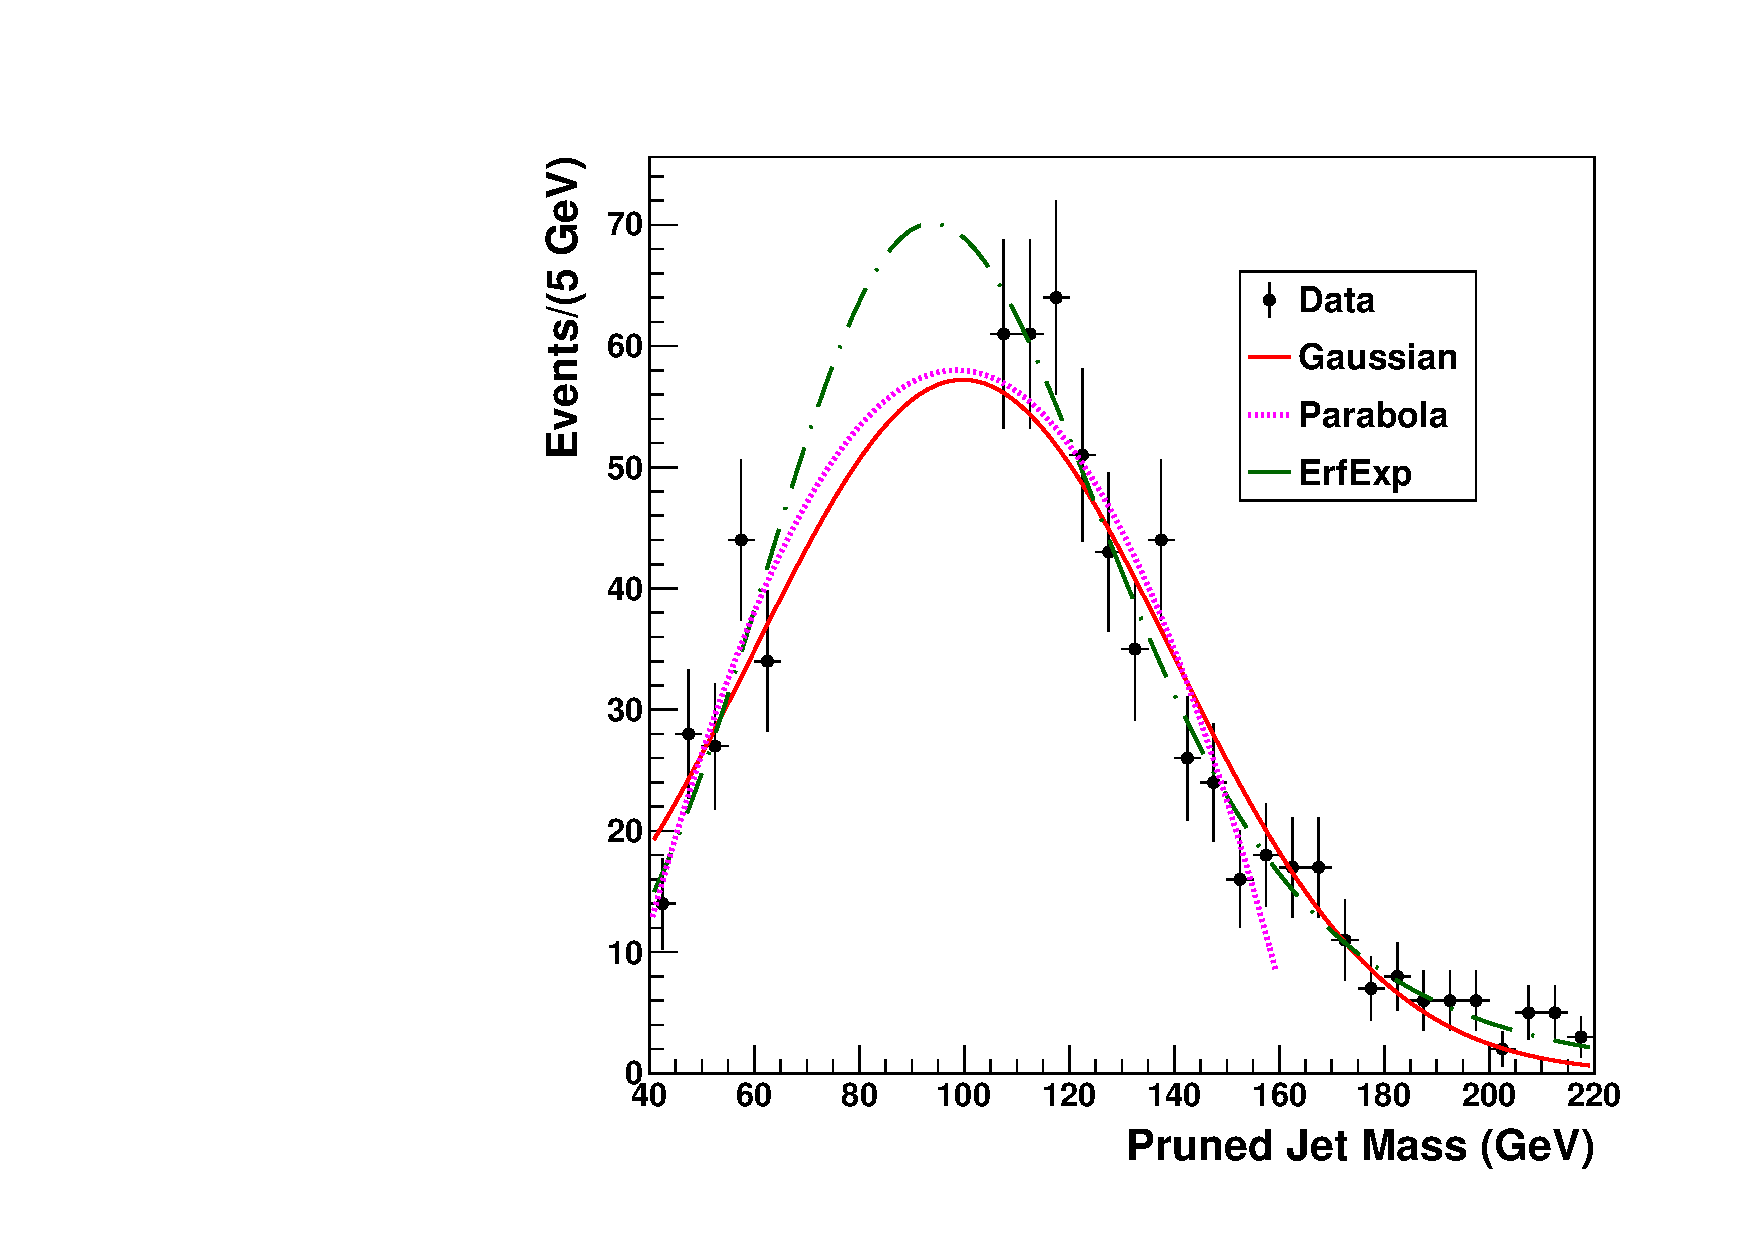
\includegraphics[width=200pt]{figures/systUnc/UncNormalHP.pdf} &
  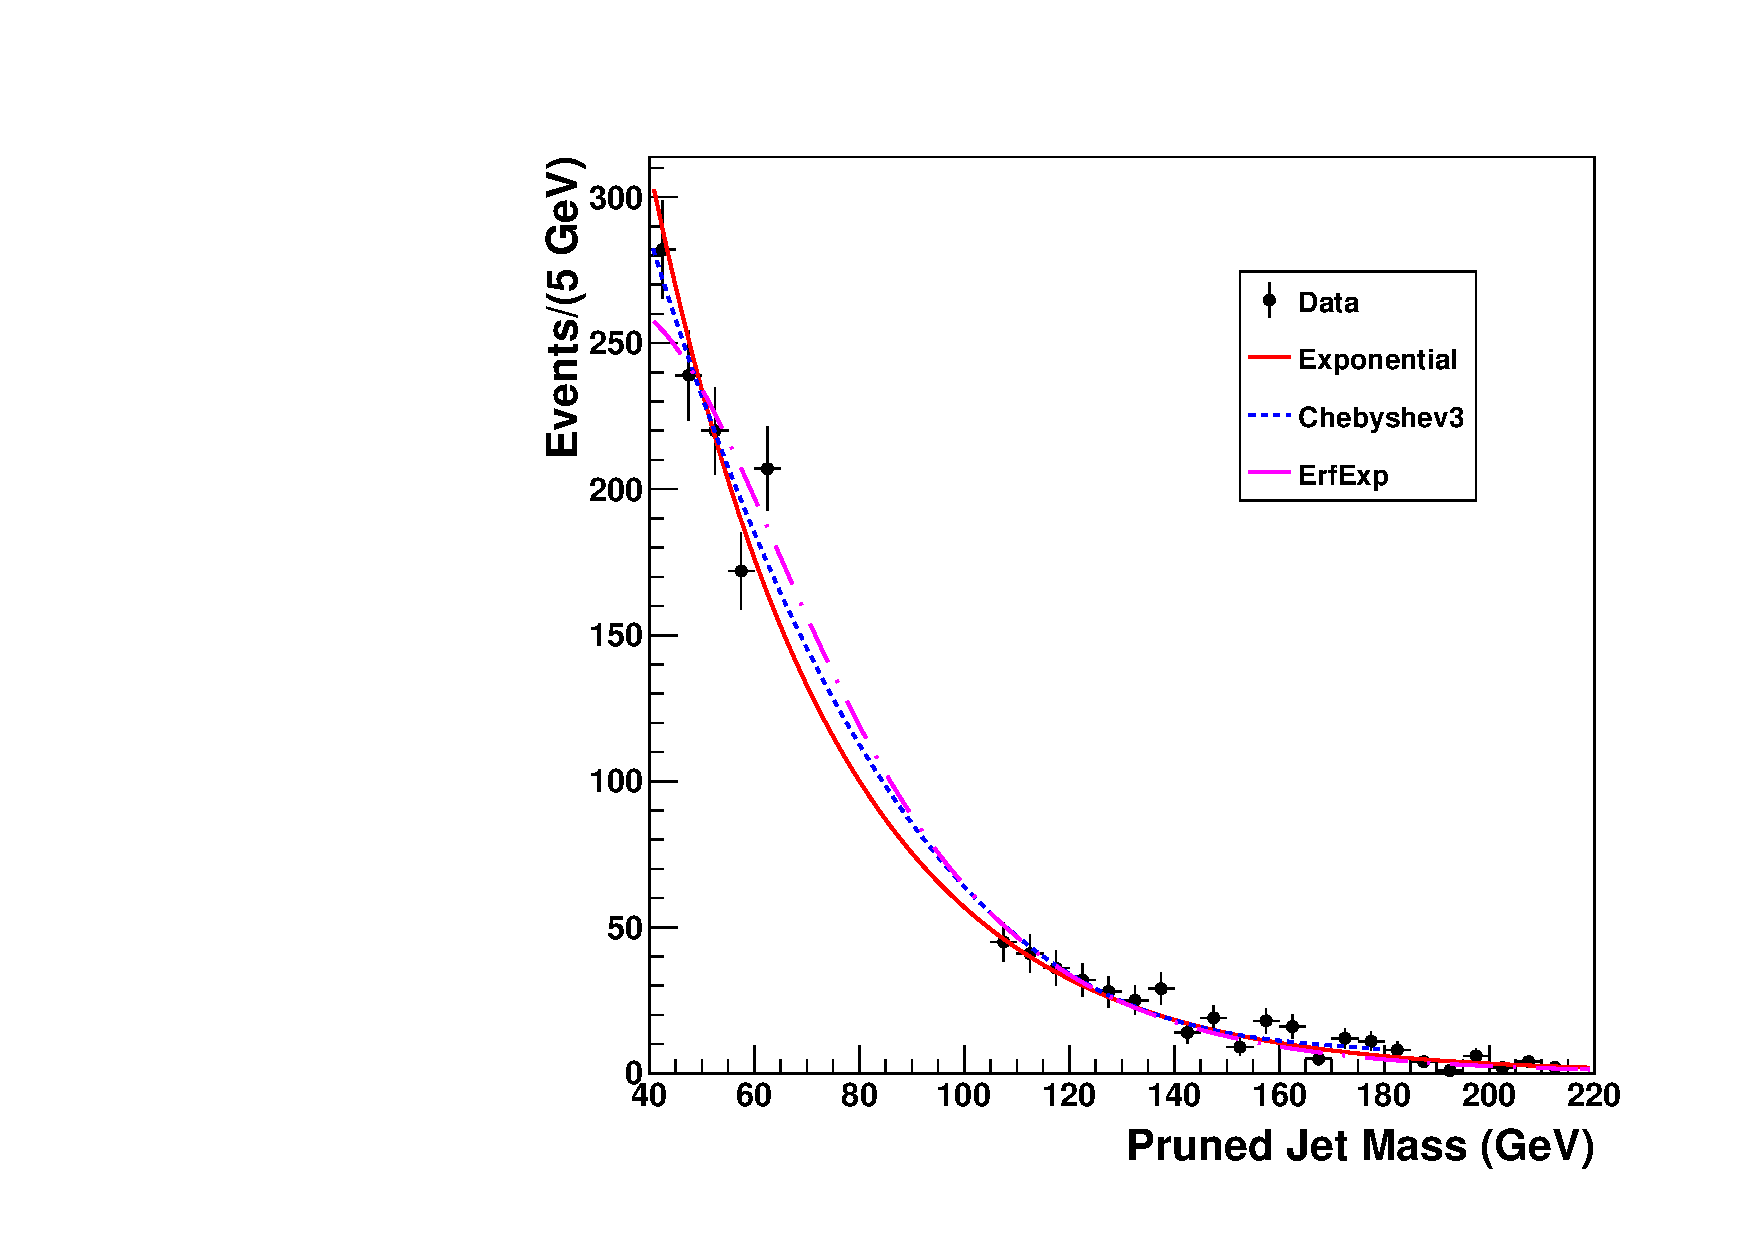
\includegraphics[width=200pt]{figures/systUnc/UncNormalLP.pdf}\\
\end{tabular}
\label{fig:fitprunedData}
\end{figure}

\begin{table}[h]
\footnotesize 
\begin{center}
\caption{Signal yields for different template functions. We show some fractions in function of the largest(l) and smallest(s) yields values. The final uncertainty ($\delta$) is calculated as the average of the two fractions.}
\label{tab:backyields2}
\begin{tabular}{ccccccccc} \hline
Category  & Gaussian & Parabola & ErfExp & Exponential & Chebychev3 & $(l-s)/s$ & $(l-s)/l$ & $\delta$ \\ \hline
HP & 412 & 430 & 507 & - & - & 23$\%$ & 18$\%$ &  20.5$\%$ \\
LP & -  & - & 732 & 817 & 858 & 17$\%$  & 14$\%$ & 15.5$\%$ \\ \hline
\end{tabular}
\end{center}
\end{table}

\section{Integrated Luminosity}\label{sys_uncert_lumi}
For the luminosity we are considering a systematic uncertainty of 2.7$\%$. This is related with the uncertainty on the number of signal events passing the final selection and is fully correlated in all the categories.

\section{Jet Substructure Scale Factors}\label{sys_uncert_jetSub}
The V-tagging efficiency scale factors for 76X were derived in \cite{CMS-AN-16-215}. These scale factors are applied to the signal yields and their uncertainty which are anti-correlated taken as systematic.

\begin{table}[h]
\small
\begin{center}
\caption{V-tagging scale factors and their systematics uncertainties for each category.}
\label{tab:VtagSF}
\begin{tabular}{ccc} \hline
Category  & Scale factor & Systematic Uncertainty \\ \hline
HP & 0.942 & 1.067/0.933 \\
LP & 1.268  & 0.74/1.26 \\ \hline
\end{tabular}
\end{center}
\end{table}


\section{QCD scale}
The impact of the systematic uncertainties due to the factorization and renormalization scales on the signal efficiency are evaluated using the weight values provided in the MC samples. The scale uncertainties are studied by varying the renormalization and factorization scales independently by a factor 1/2 and 2. The associated systematic uncertainty due to the shift of the signal peak varies between 0.2$\%$ and 0.5$\%$ and 12$\%$ for the subdominant backgrounds. The figure \ref{fig:QCDuncert} show the QCD scale systematic uncertainties for different signal mass points.

\begin{figure}[!ht]
\caption{ Systematic uncertainties due to the factorization and renormalization scales for different signal mass points.}
\begin{center}
  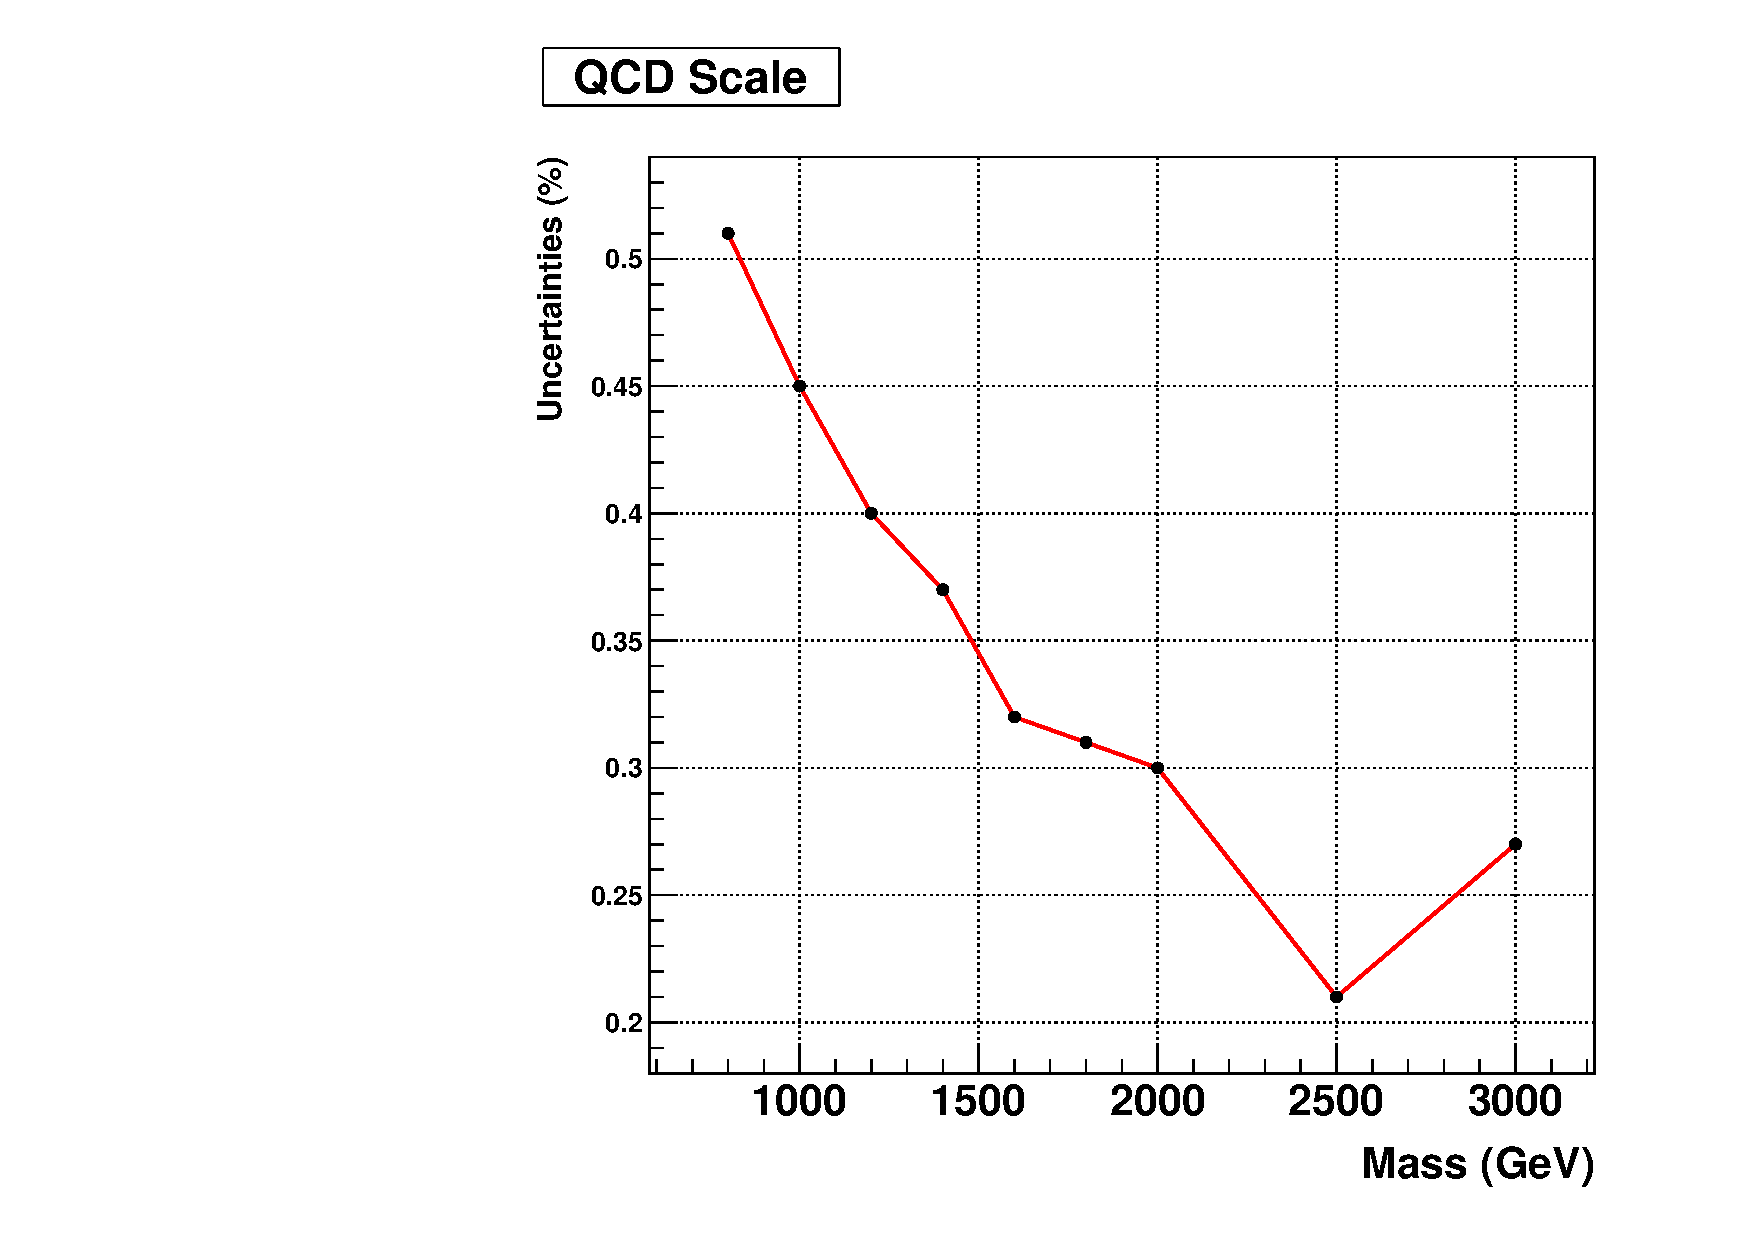
\includegraphics[width=230pt]{figures/SystUncert/UncertQCD.pdf}
\end{center}
\label{fig:QCDuncert}
\end{figure}

\subsection{PDF}

The PDF Systematic uncertainties for the NNPDF3.0 set was calculated using the PDF4LHC prescription \cite{Butterworth:2015oua}. The standard deviation was obtained as the RSM value of the weights per event. The evaluation was performed by raising and lowering the respective uncertainty by one standard deviation. The associated systematic uncertainty due to the shift of the signal peak varies between 8$\%$ and 18$\%$ for signal samples and 17$\%$ for subdominant backgrounds . The figure \ref{fig:PDFuncert} show the PDF systematic uncertainties for different signal mass points.

\begin{figure}[!ht]
\caption{ Left : Transverse Mass of the candidate with the nominal value of the PDF. Also we show the scale up and down in one standard deviation for a signal of 2 TeV. Right: PDF systematic uncertainties for different signal mass point. }
\begin{tabular}{cc}
  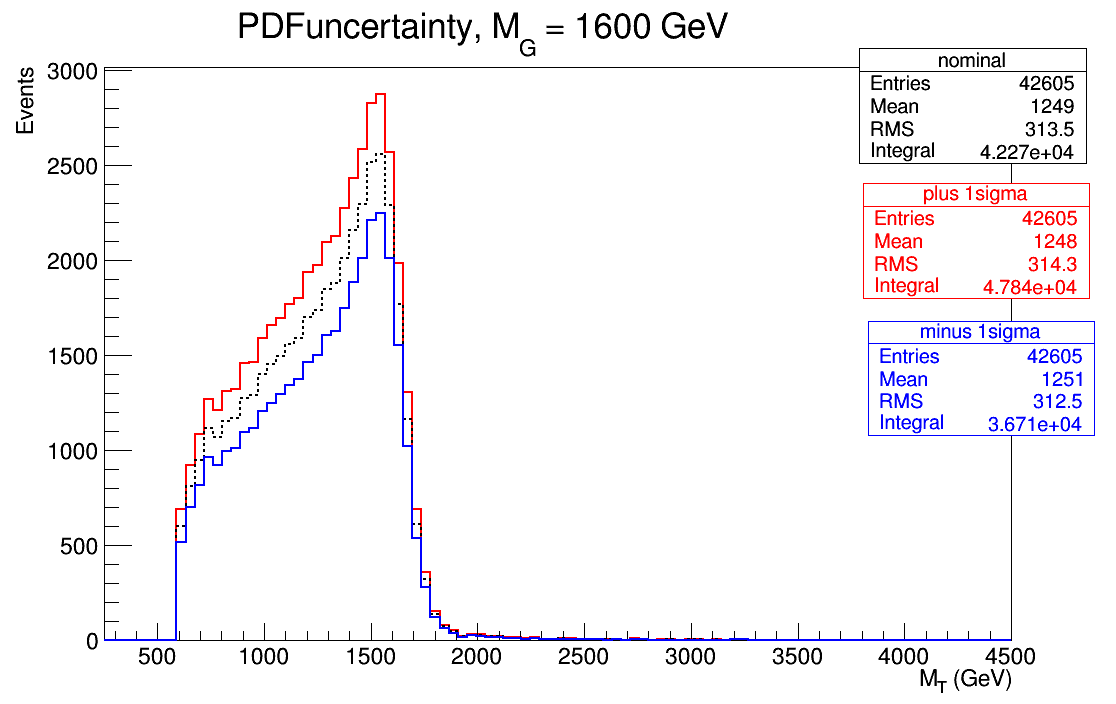
\includegraphics[height=7cm,width=9cm]{figures/SystUncert/UncertPDF.png} &
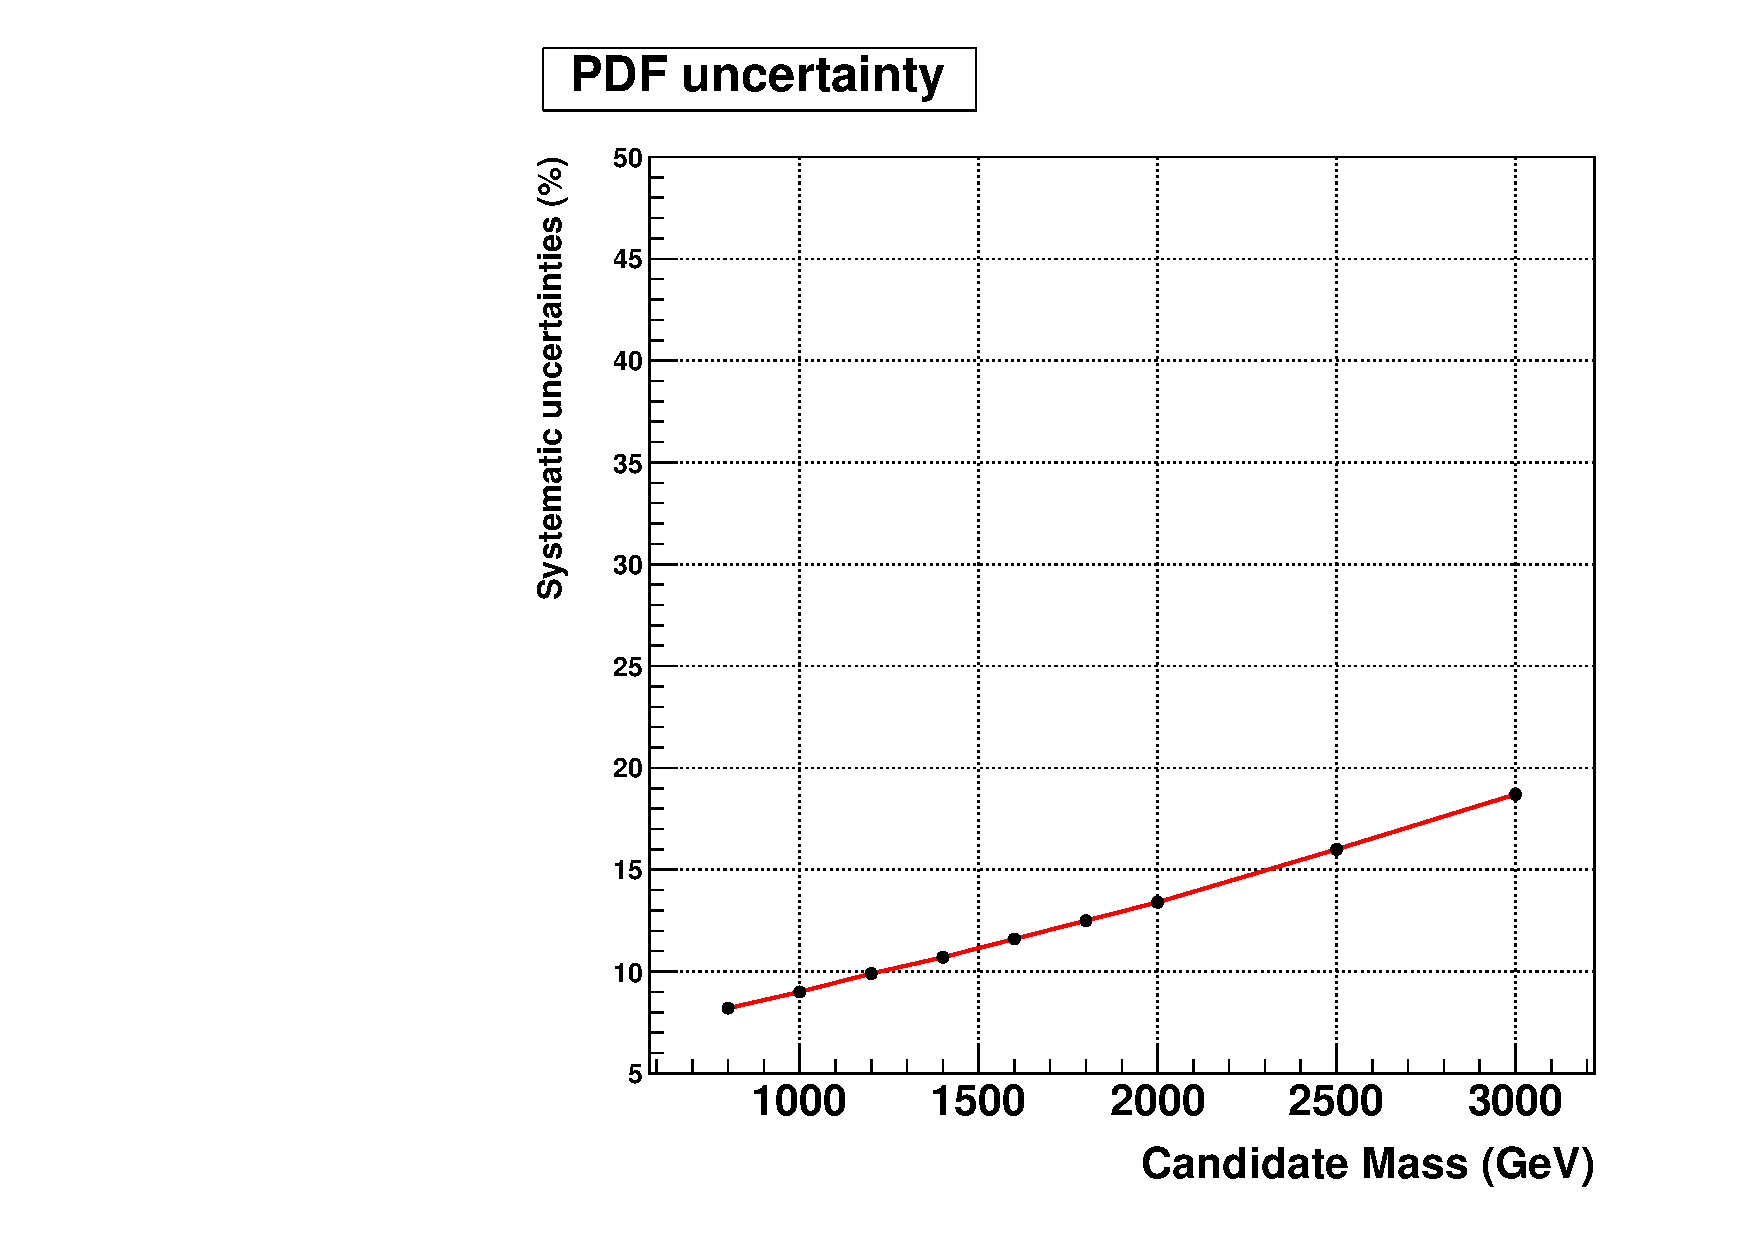
\includegraphics[width=220pt]{figures/SystUncert/PDFuncert.pdf}\\
\end{tabular}
\label{fig:PDFuncert}
\end{figure}

\section{Trigger SF}

We estimate the uncertainty of the trigger SF from the ratio between the efficiency measured in Data and the efficiency measured in MC:
\begin{eqnarray}
\text{ratio} = \dfrac{\text{efficiency}_{\text{Data}}}{\text{efficiency}_{\text{MC}}} 
\end{eqnarray}
The uncertainty in the ratio is given by:
\begin{eqnarray}
 \Delta \text{ratio} = \text{ratio} \times \sqrt{  \left(\dfrac{ \Delta y }{y} \right)^{2}_{\text{eff-Data}} + \left(\dfrac{ \Delta y }{y} \right)^{2}_{\text{eff-MC}} } 
\end{eqnarray}
where $y$ give the value of the efficiency and $\Delta y$ it uncertainty. We consider the SF as a weight in the event and then we define some variations:
\begin{eqnarray}
 \text{triggerWeight} = \text{ratio}
\end{eqnarray}
\begin{eqnarray}
 \text{triggerWeightup} = \text{ratio} +  \Delta \text{ratio}
\end{eqnarray}
\begin{eqnarray}
 \text{triggerWeightdown} = \text{ratio} -  \Delta \text{ratio}
\end{eqnarray}
Then we will estimate the impact in the transverse mass in signal after apply the trigger weights (up and down), as it can be observed in the figure \ref{fig:Trigguncert}.
\begin{figure}[!ht]
\caption{Systematic uncertainties due to the trigger SF for different signal mass points. }
\begin{center}
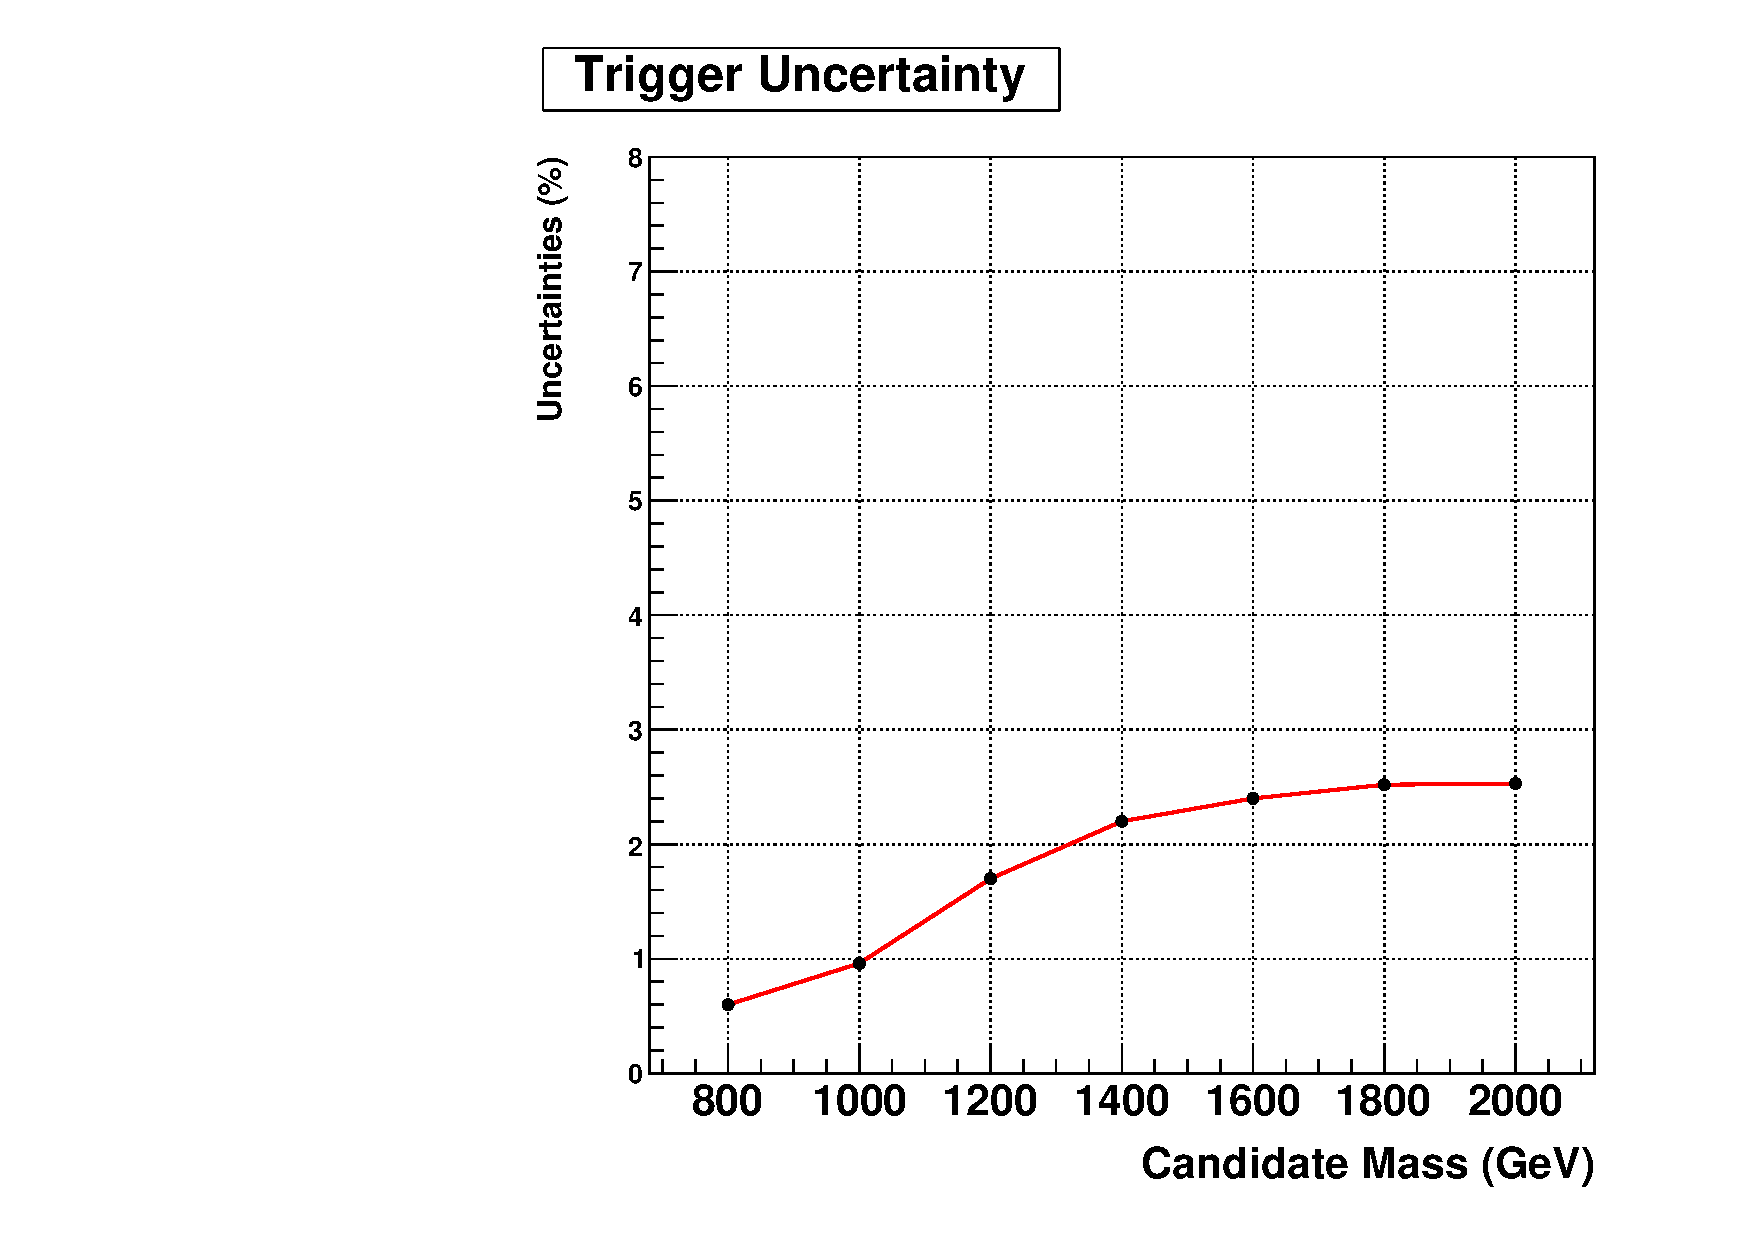
\includegraphics[width=250pt]{figuresARC/triggerWeight/TriggerUncert.pdf}
\end{center}
\label{fig:Trigguncert}
\end{figure}
The associated systematic uncertainty due to the trigger SF is around 2.5$\%$.

\section{B-tagging}

The effect of the b-tagging uncertainty is evaluated by varying the CSV scale factors (up and down) for the respective flavor. The associated systematic uncertainty due to the shift of the signal peak varies between 0.02$\%$ and 0.04$\%$. The figure \ref{fig:BTAGuncert} show the evaluation of the uncertainty for different mass points.

\begin{figure}[!ht]
\caption{ Left : Systematic uncertainties due to b-tagging uncertainty SF for different signal mass points. Right : Number of b-tag jets for different signal mass points.}
\begin{tabular}{cc}
 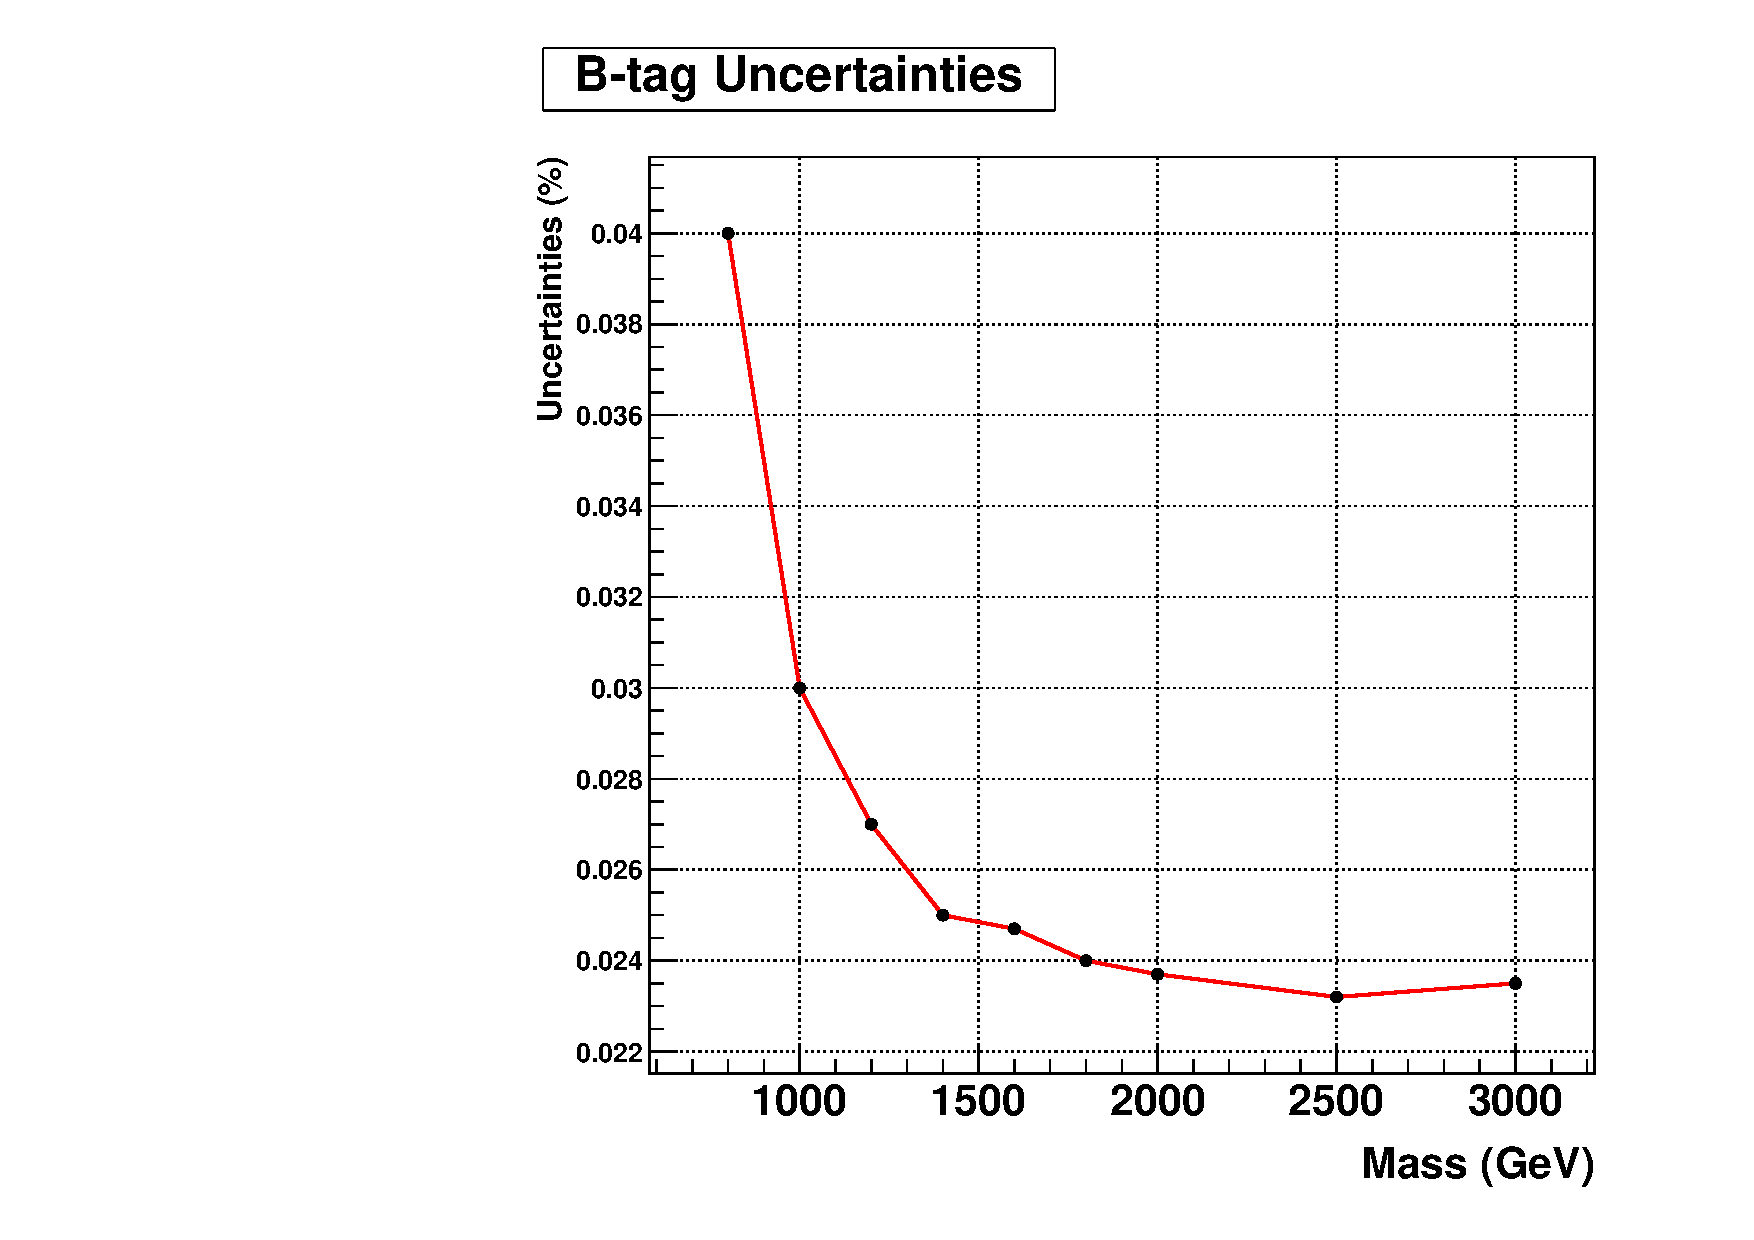
\includegraphics[width=220pt]{figures/SystUncert/UncertBTAG.pdf} &
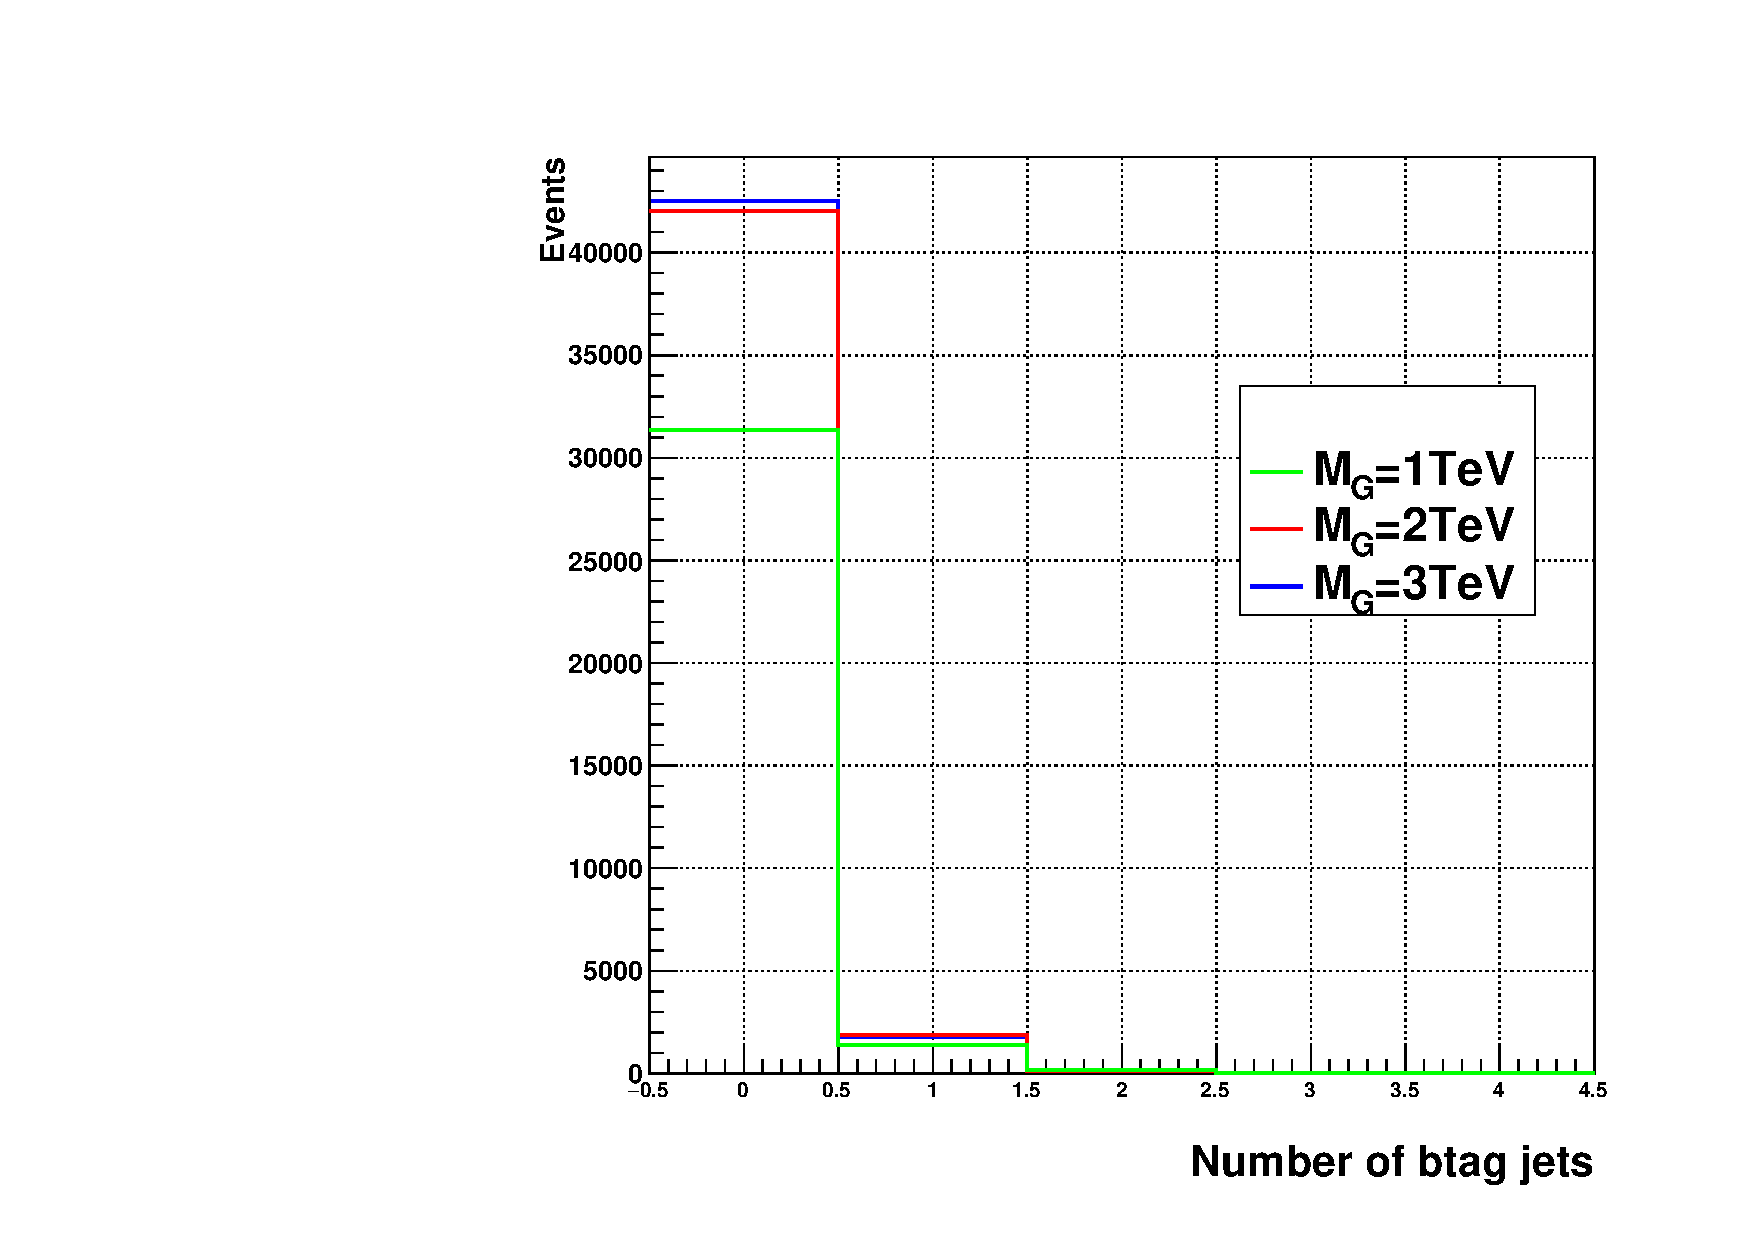
\includegraphics[width=220pt]{figures/SystUncert/Nbtagjets.pdf}\\
\end{tabular}
\label{fig:BTAGuncert}
\end{figure}

In the fiure \ref{fig:BTAGuncertback} we show the eveluation for the backgrounds : Z+jets, W+jets and TTbar. In case of the TT bar the systematic uncertainty is 1 $\%$, and for Z/W + jets 0.05 $\%$. 

\begin{figure}[!ht]
\caption{ Systematic uncertainties due to b-tagging uncertainty SF. Top : Nominal and scale up/down variations values in the transverse mass distribution for (Left) $t\bar{t}$ sample (right) W+jets sample .Bottom : (left) Z+jets sample (right)  Number of b-tag jets for different backgrounds models.}
\begin{tabular}{cc}
 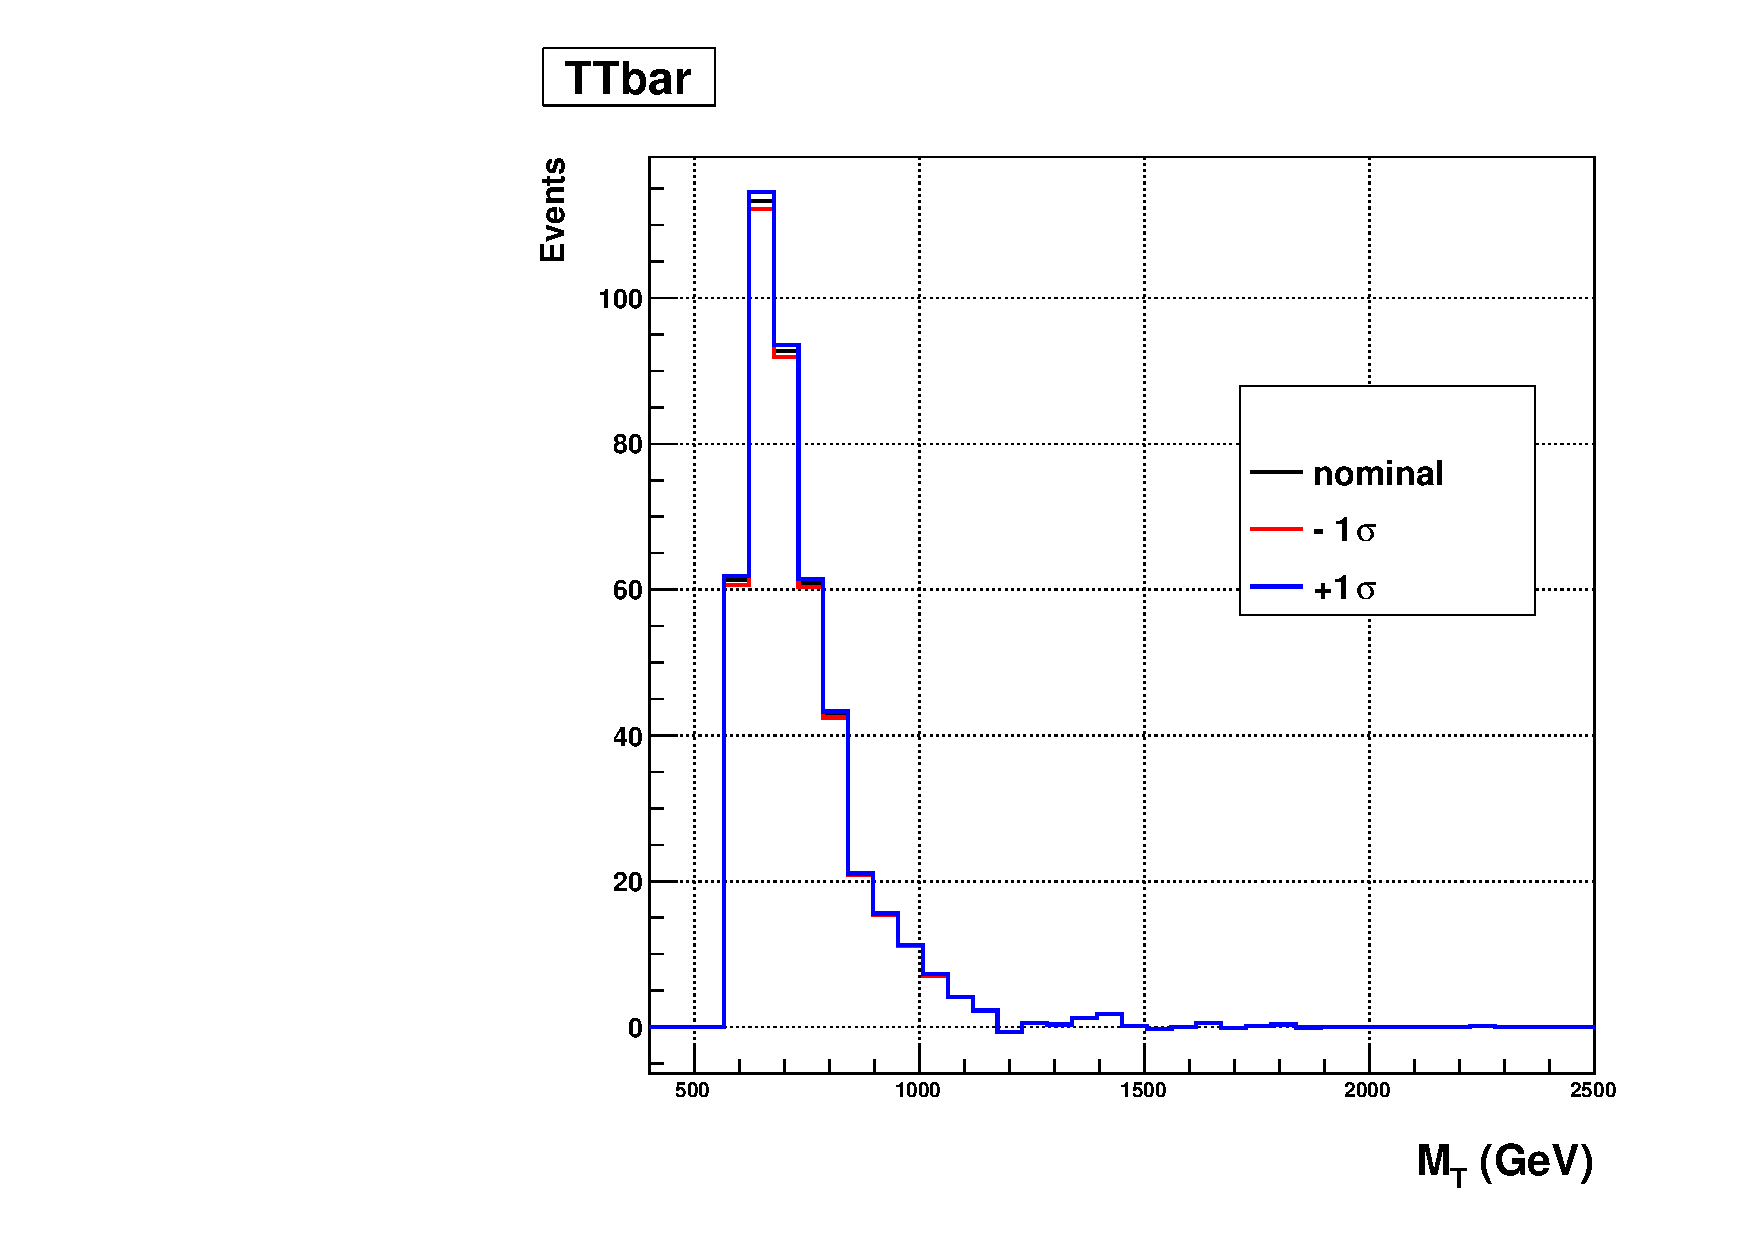
\includegraphics[width=220pt]{figures/SystUncert/btagjetsTTjets.pdf} &
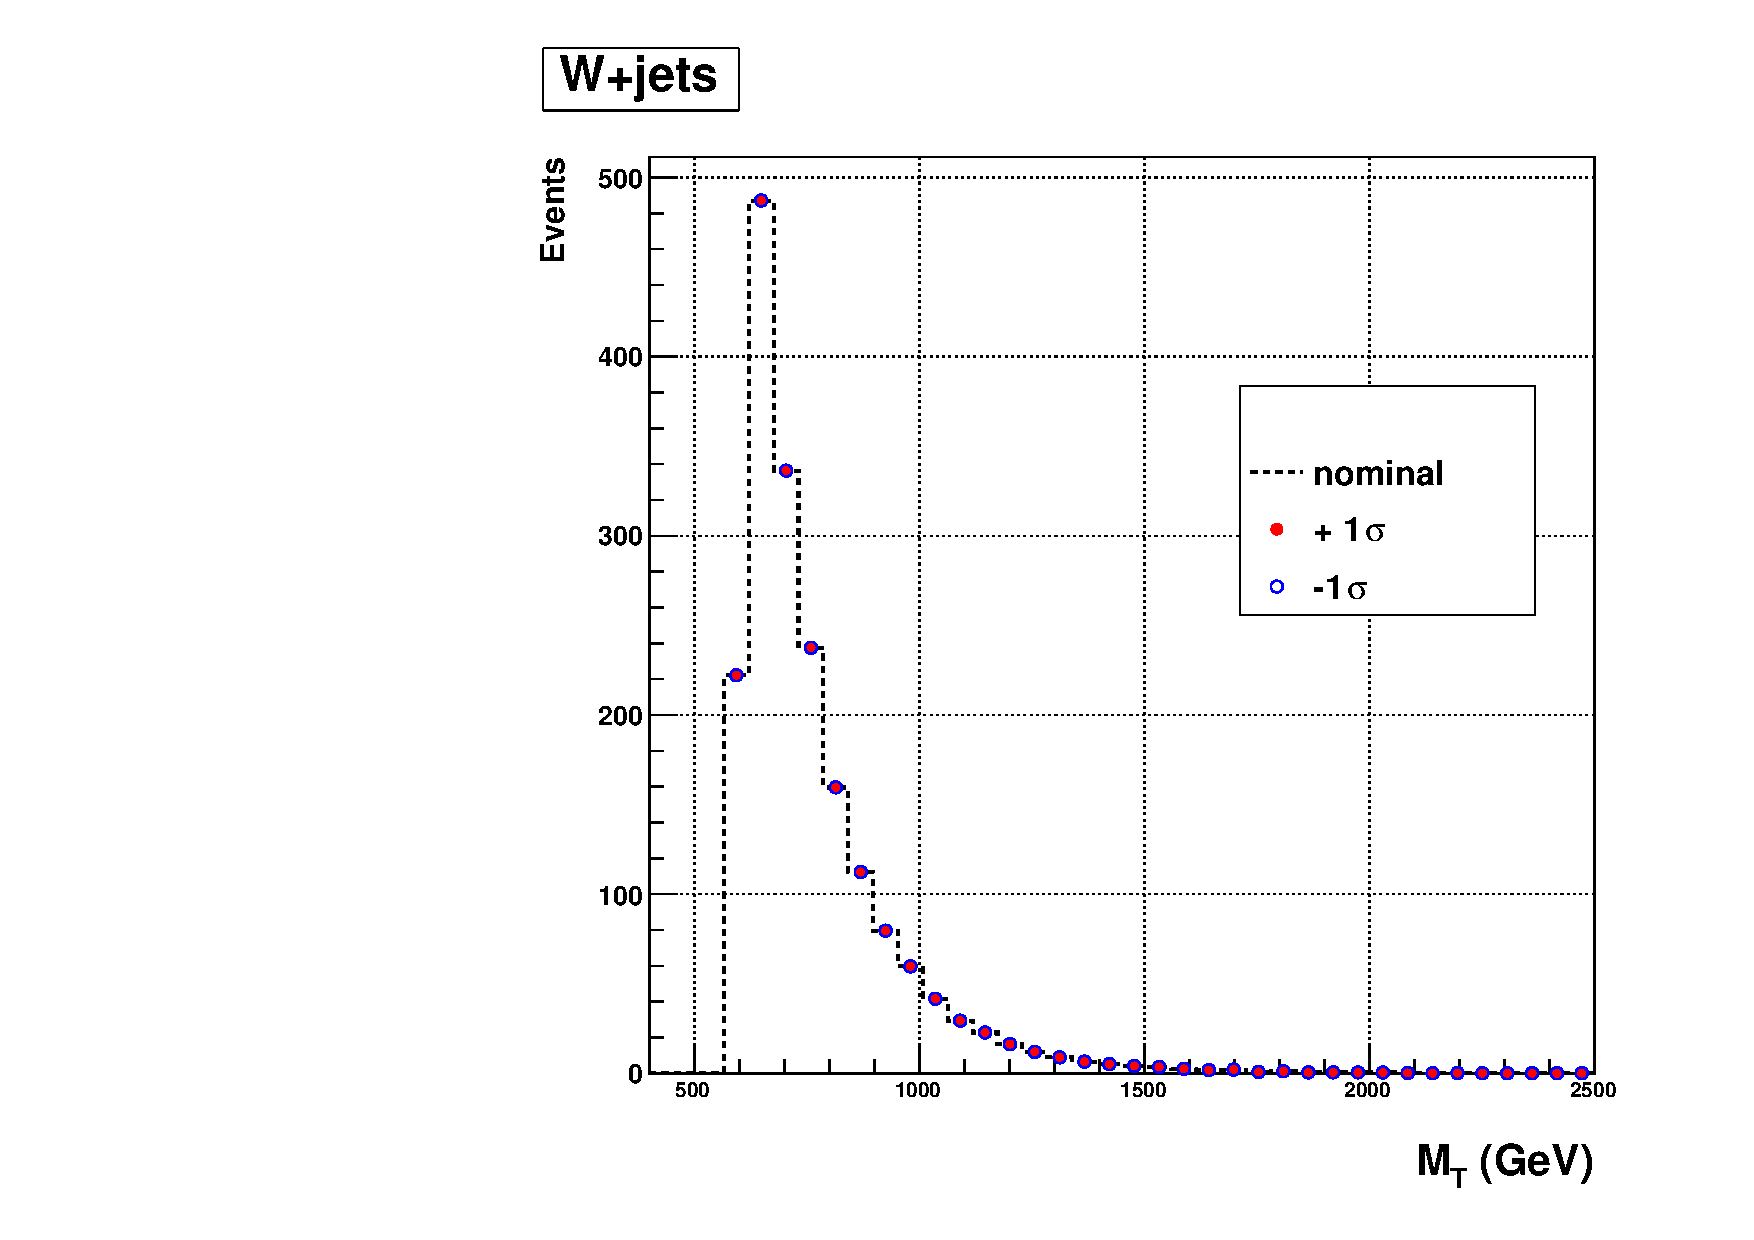
\includegraphics[width=220pt]{figures/SystUncert/btagjetsWjets.pdf}\\
 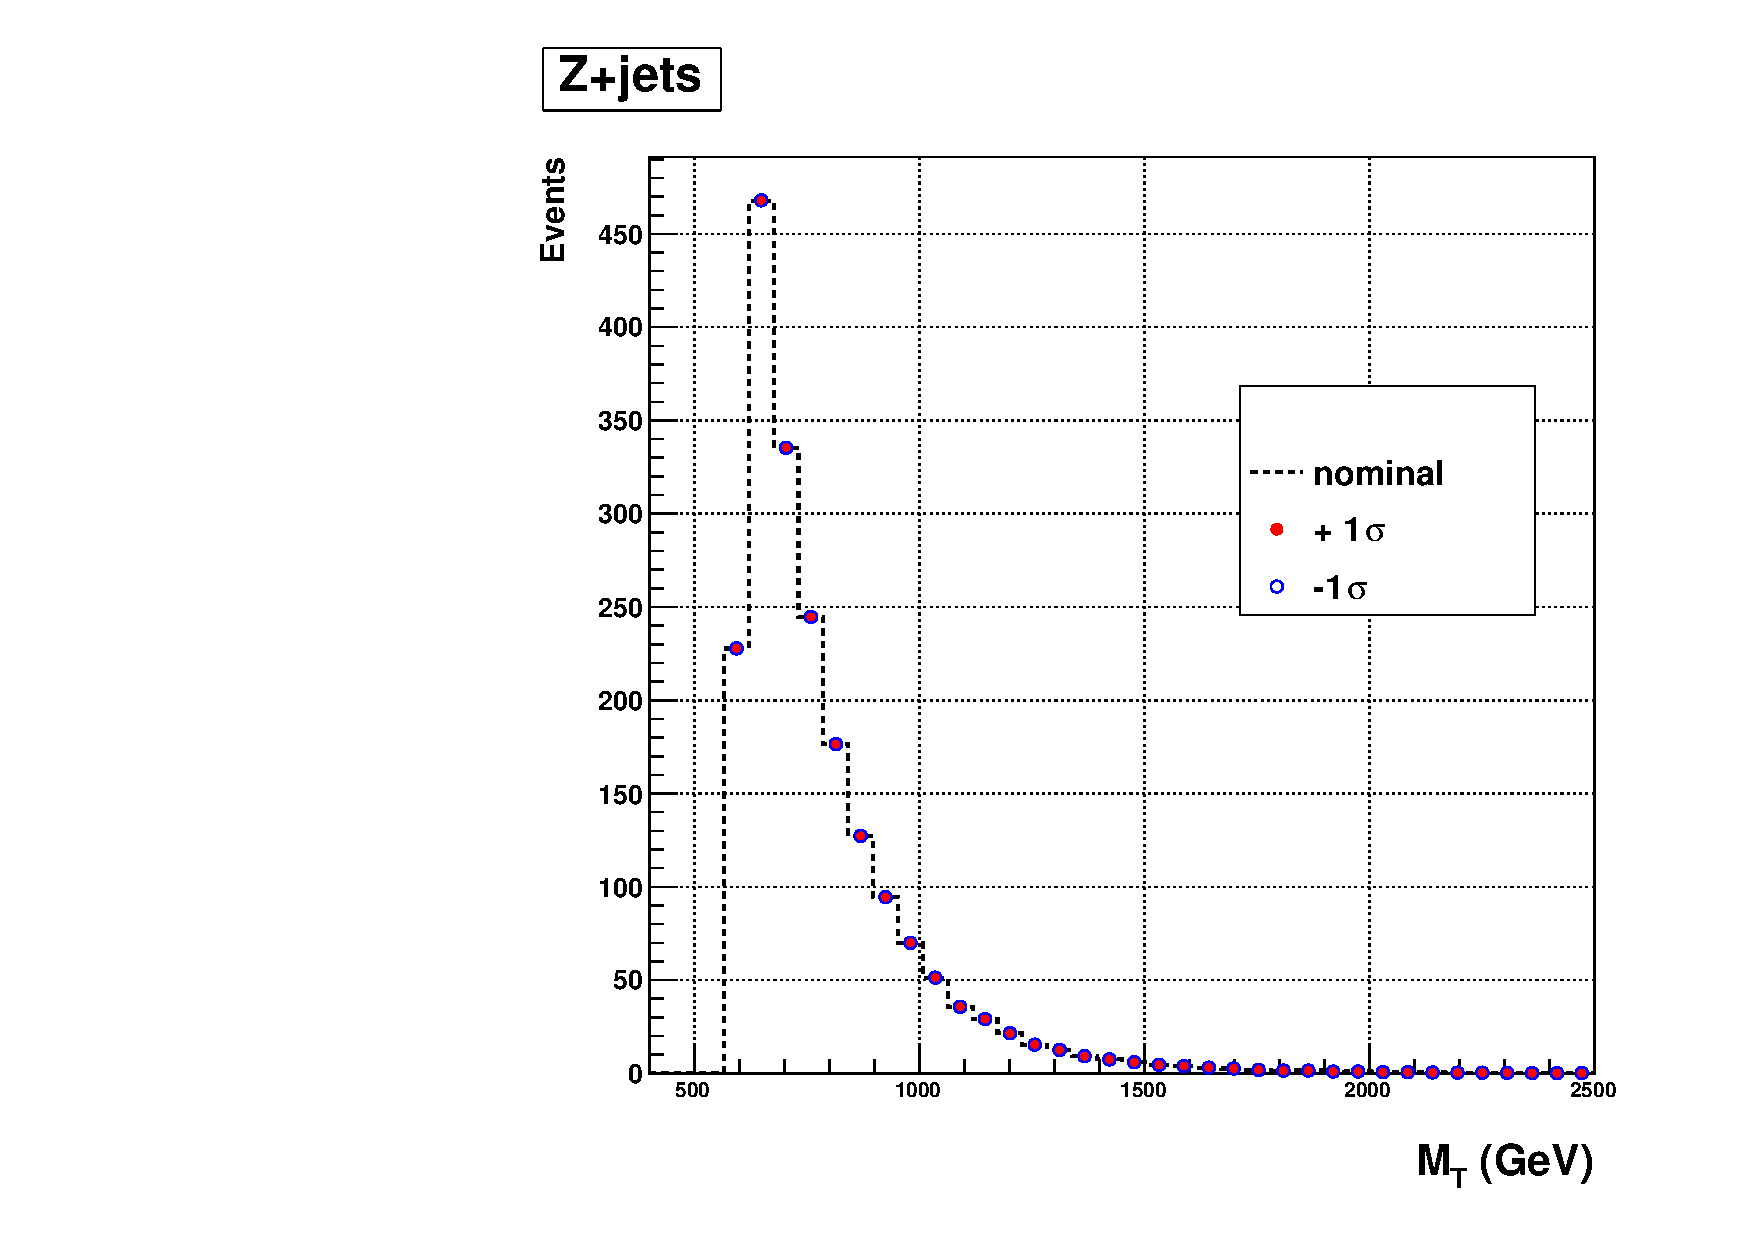
\includegraphics[width=220pt]{figures/SystUncert/btagjetsZjets.pdf} &
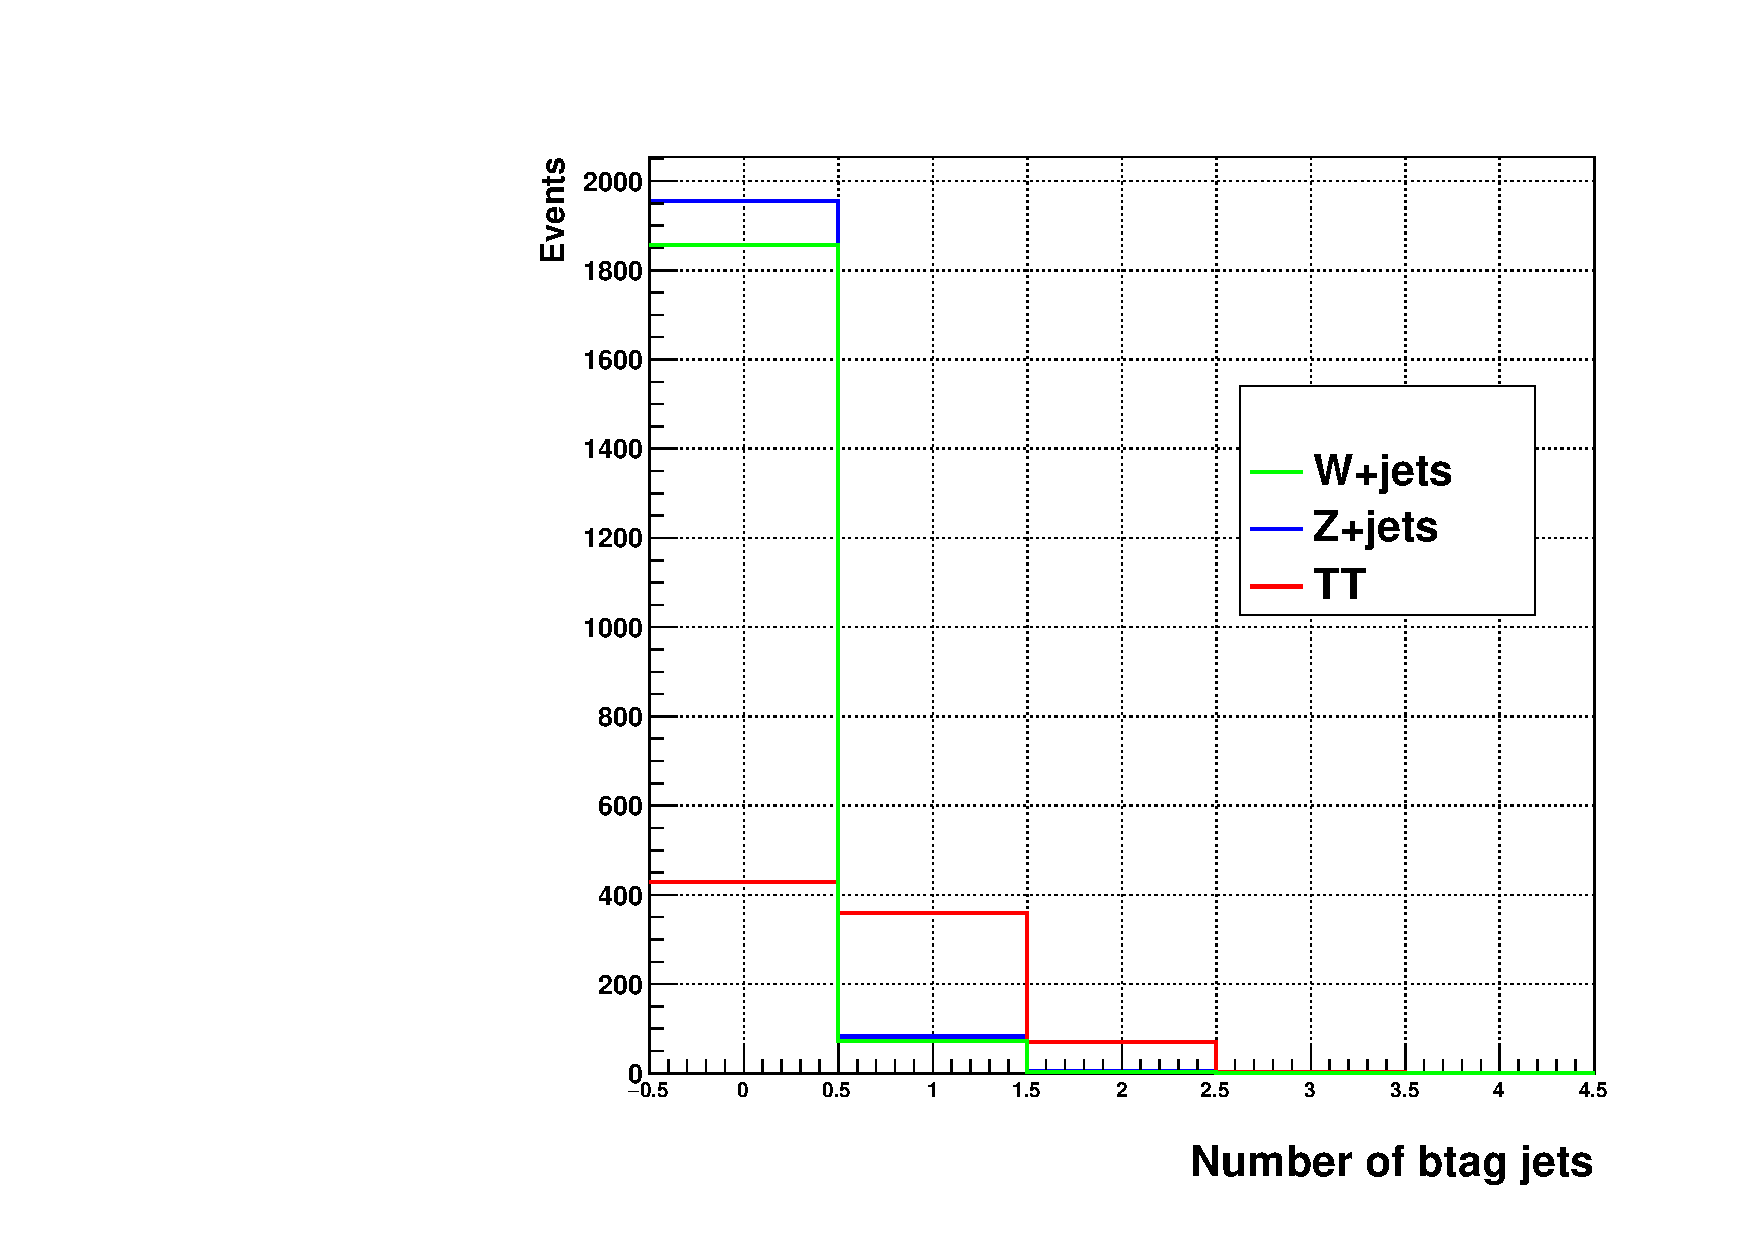
\includegraphics[width=220pt]{figures/SystUncert/Nbtagjetsback.pdf}\\
\end{tabular}
\label{fig:BTAGuncertback}
\end{figure}


\section{Pile-up}

For the PU uncertainties we test over different minbias cross-section (72mb, 69mb, 66mb) to obtain the pileup weights. In the figure \ref{fig:PUuncert}  we show different scenarios for a signal mass of 2 TeV. In this case the unceratinty is of 0.02$\%$ for signal and 2.3$\%$ for the subdominant backgrounds. 

\begin{figure}[!ht]
\caption{ Systematic uncertainties on the pile-up due to different minbias cross-section for a signal mass of 2 TeV.}
\begin{center}
  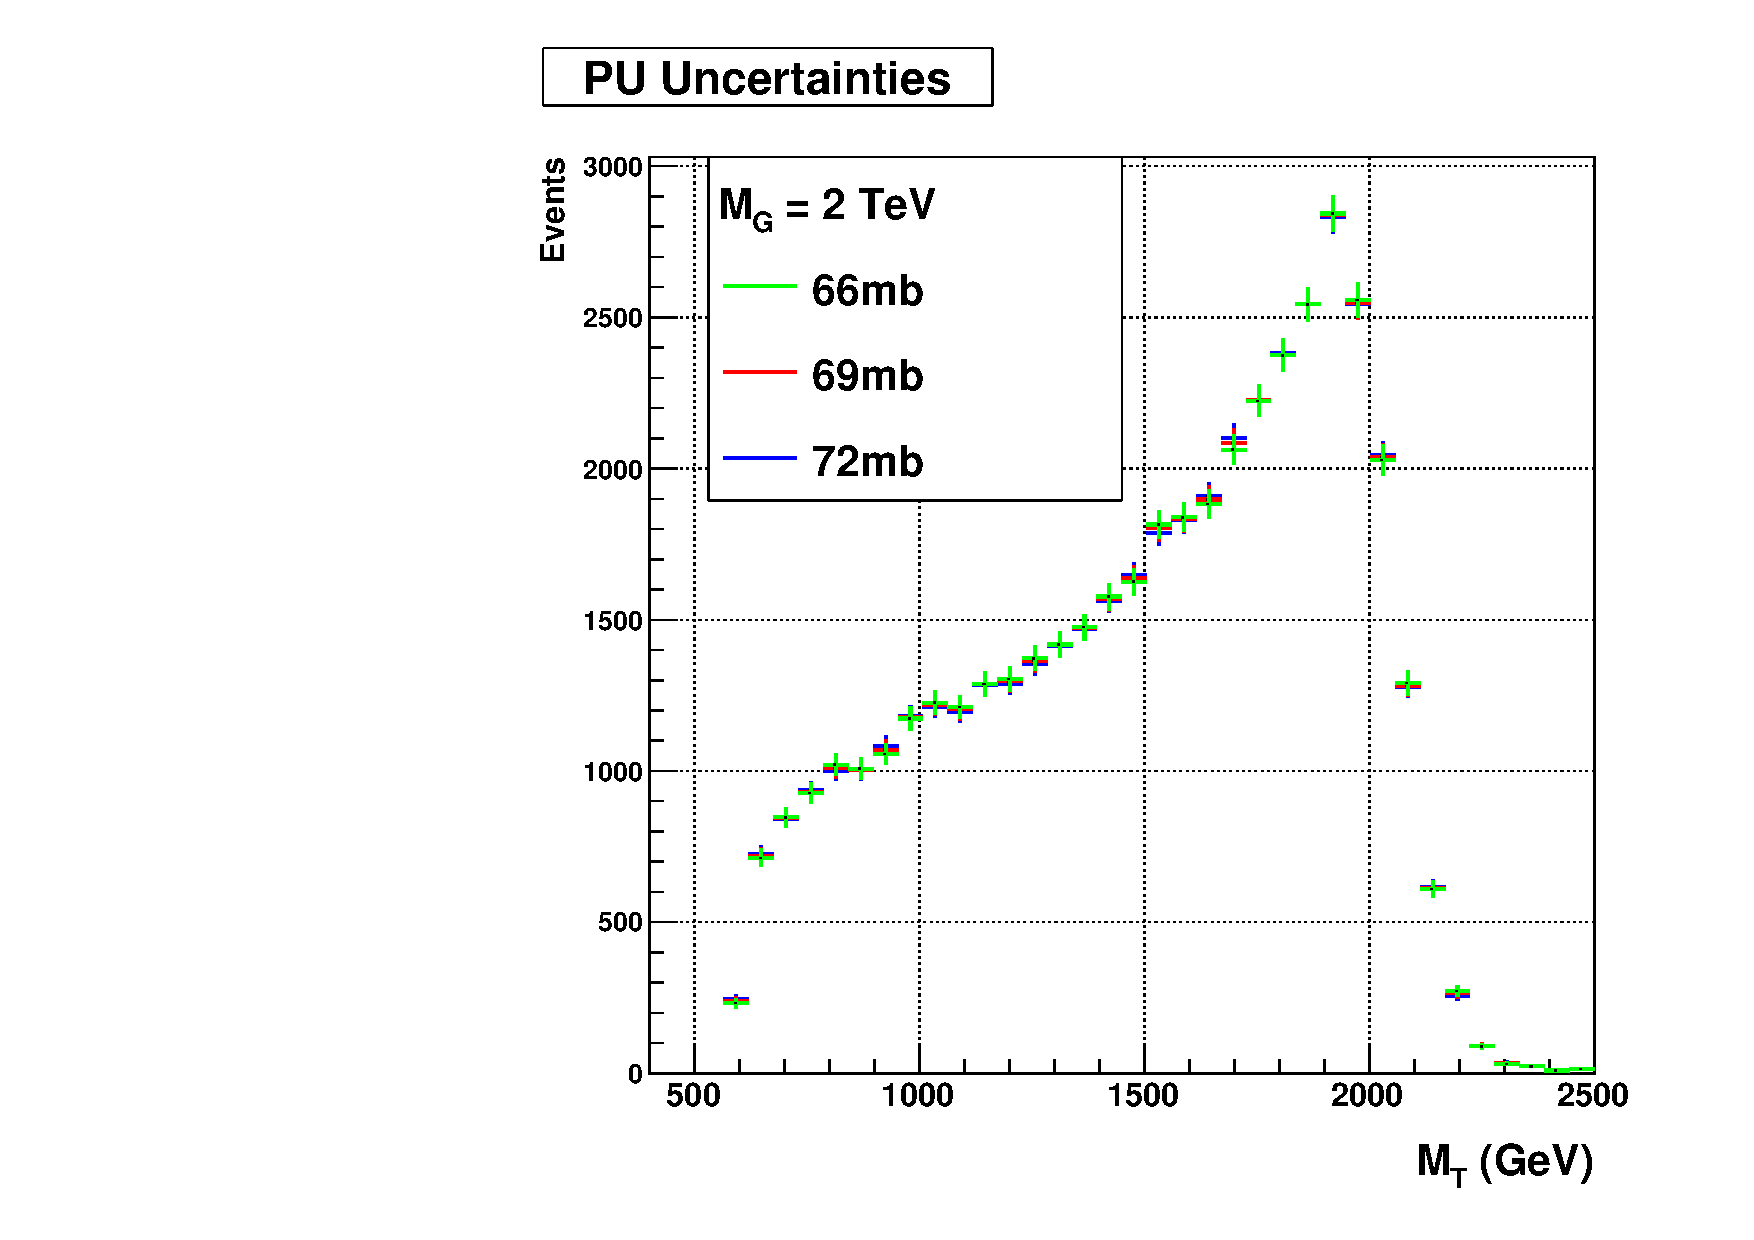
\includegraphics[width=230pt]{figures/SystUncert/UncertPU.pdf}
\end{center}
\label{fig:PUuncert}
\end{figure}


\section{Jet Energy Corrections}

The impact of the JEC uncertainties are evaluated scaling up and down the jet $\pt$. We consider the propagation of the JEC to the missing energy, so the variation was applied in both jets and $\MET$ (up,up) and (down,down). The associated systematic uncertainty due to the shift of the signal peak varies between 0.09$\%$ and 1.76$\%$. For the subdominant backgrounds is 3$\%$. The figure \ref{fig:JECuncert} show the JEC systematic uncertainties for different signal mass points.
\begin{figure}[!ht]
\caption{ Systematic uncertainties due to the JEC for different signal mass points.}
\begin{center}
  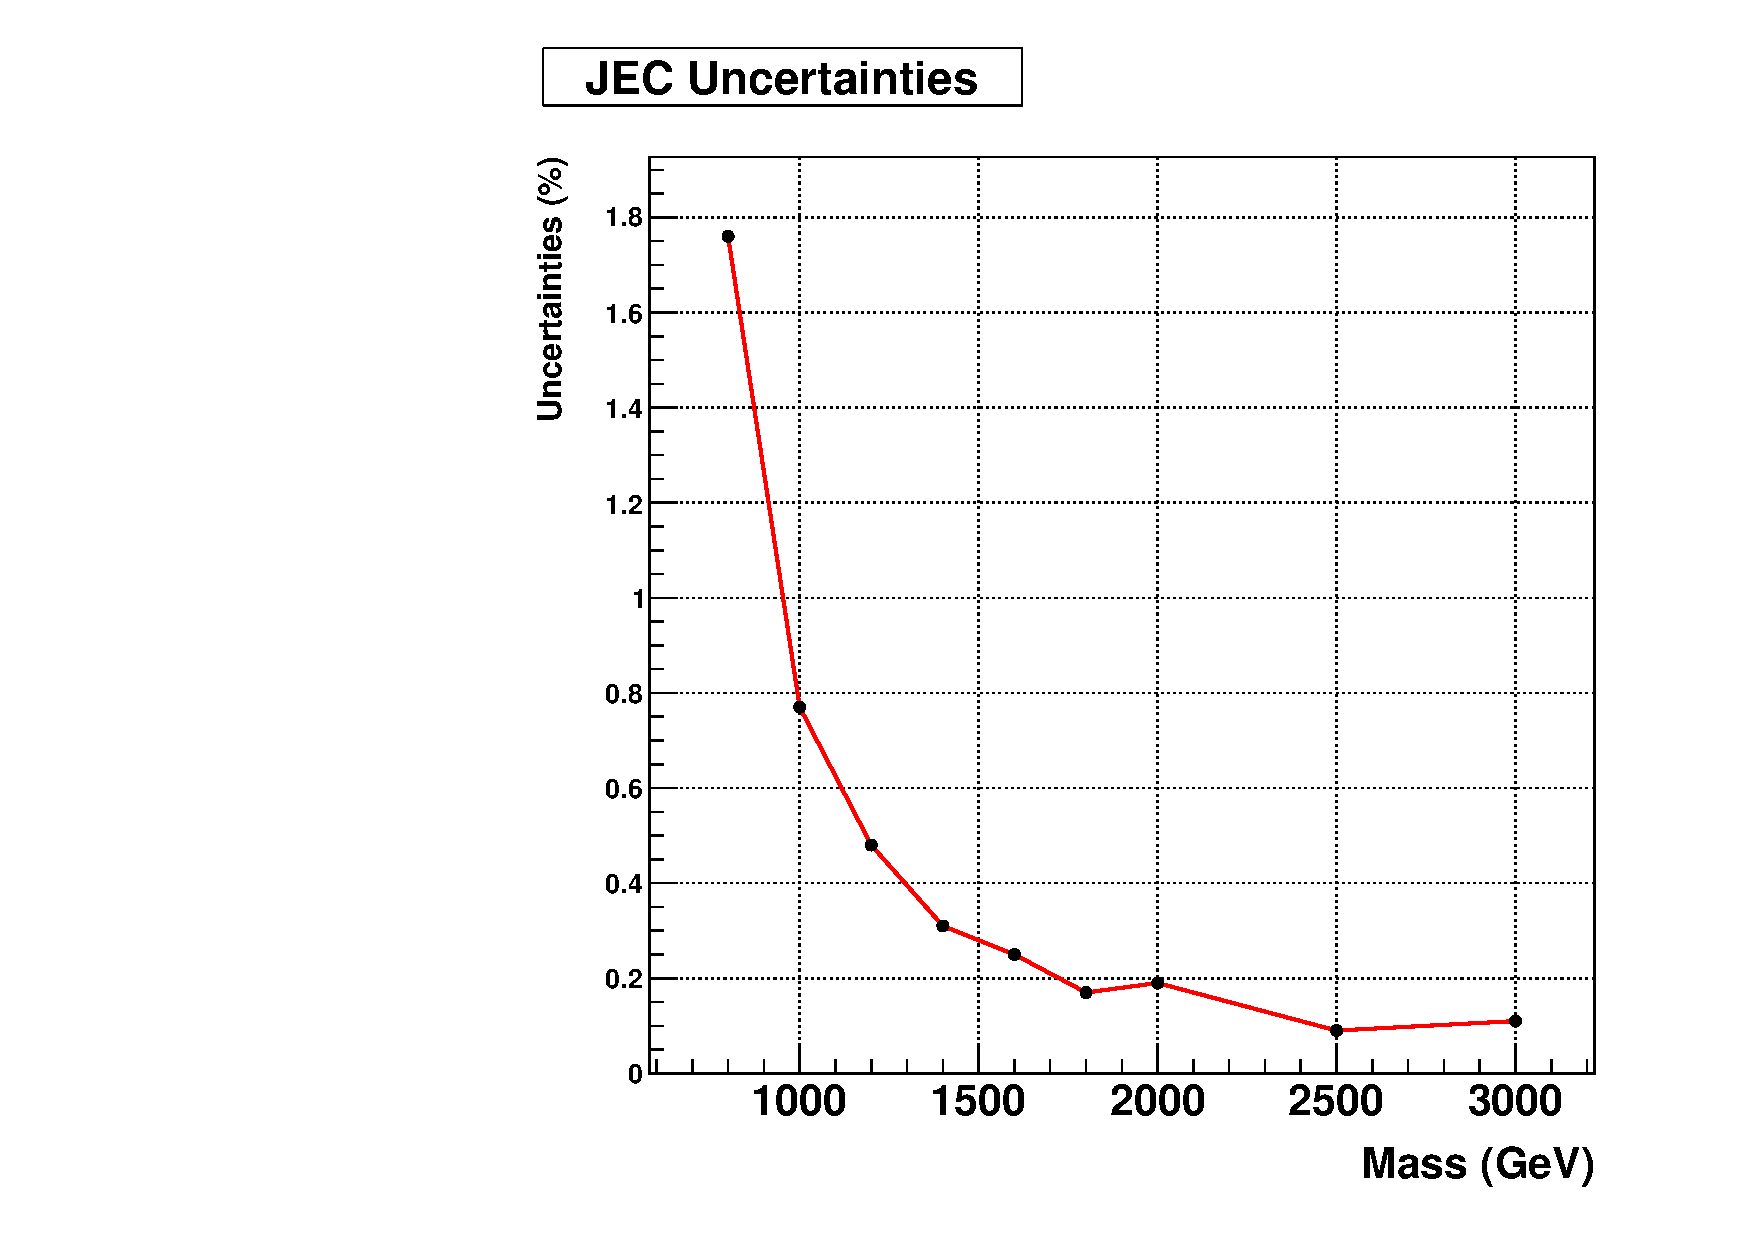
\includegraphics[width=230pt]{figures/SystUncert/UncertJEC.pdf}
\end{center}
\label{fig:JECuncert}
\end{figure}

\section{Jet Energy Resolution}

We smeared the jets using Jet energy resolution scaling factors and the uncetainties are tested by varying its value in by one standard deviation (up and down). We found that the systematic uncertainties for the Jet resolution are small ranging from 0.009$\%$ to 0.06$\%$. For the subdominant backgrounds we do not observe any significant variation.


\section{Leptons and photons ID}

The systematic uncertainties due to scale factors for leptons and photons are very small in the analysis. In the case of a signal mass of 1 TeV the propagation of the uncertainty in +/- 1 $\sigma$ gives no significant variation in the efficiency. For a mass of 3TeV the uncertainty is of 0.02$\%$. We consider these systematics negligibles.

\section{Jet mass calibration uncertainty}

As we are using a W/Z-tagger we need to consider the uncertainty in the pruned jet mass calibration. We vary the jet pruned mass calibration in order to calculate the impact on the signal selection efficiency. This was applied in the context of 76X with v2 JEC (pruned jet mass + N-subjettiness). The shift of the signal peak varies between 0.13$\%$ and 0.22$\%$. The figure \ref{fig:masscalib} show the systematic uncertainties due to the jet mass calibration for different mass points.

\begin{figure}[!ht]
\caption{ Systematic uncertainties due to jet mass calibration. Left : Nominal and scale up/down variations values in the pruned jet mass distribution for a signal point of 1000 GeV. Right  : Systematic uncertainties in $(\%)$ for different mass points.}
\begin{tabular}{cc}
 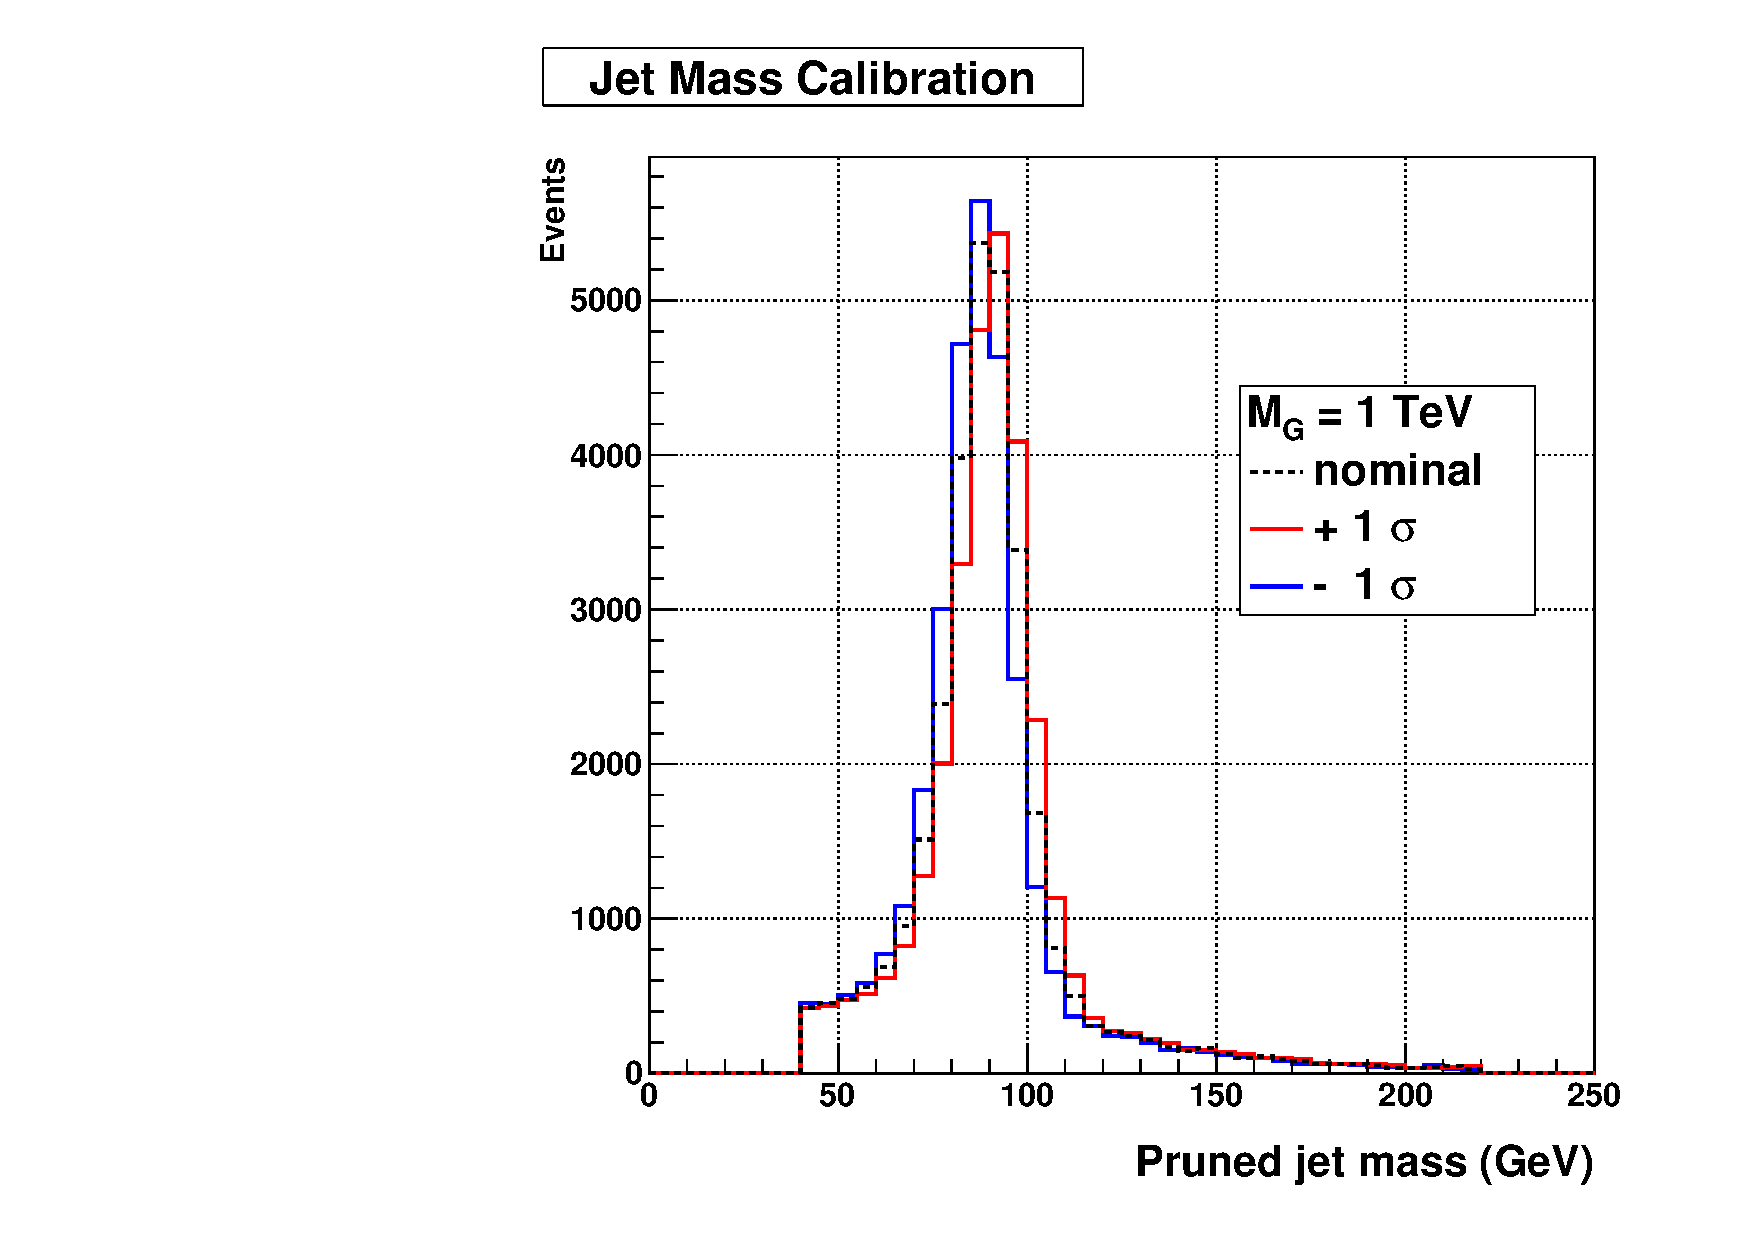
\includegraphics[width=220pt]{figures/SystUncert/JetmassScale1000.pdf} &
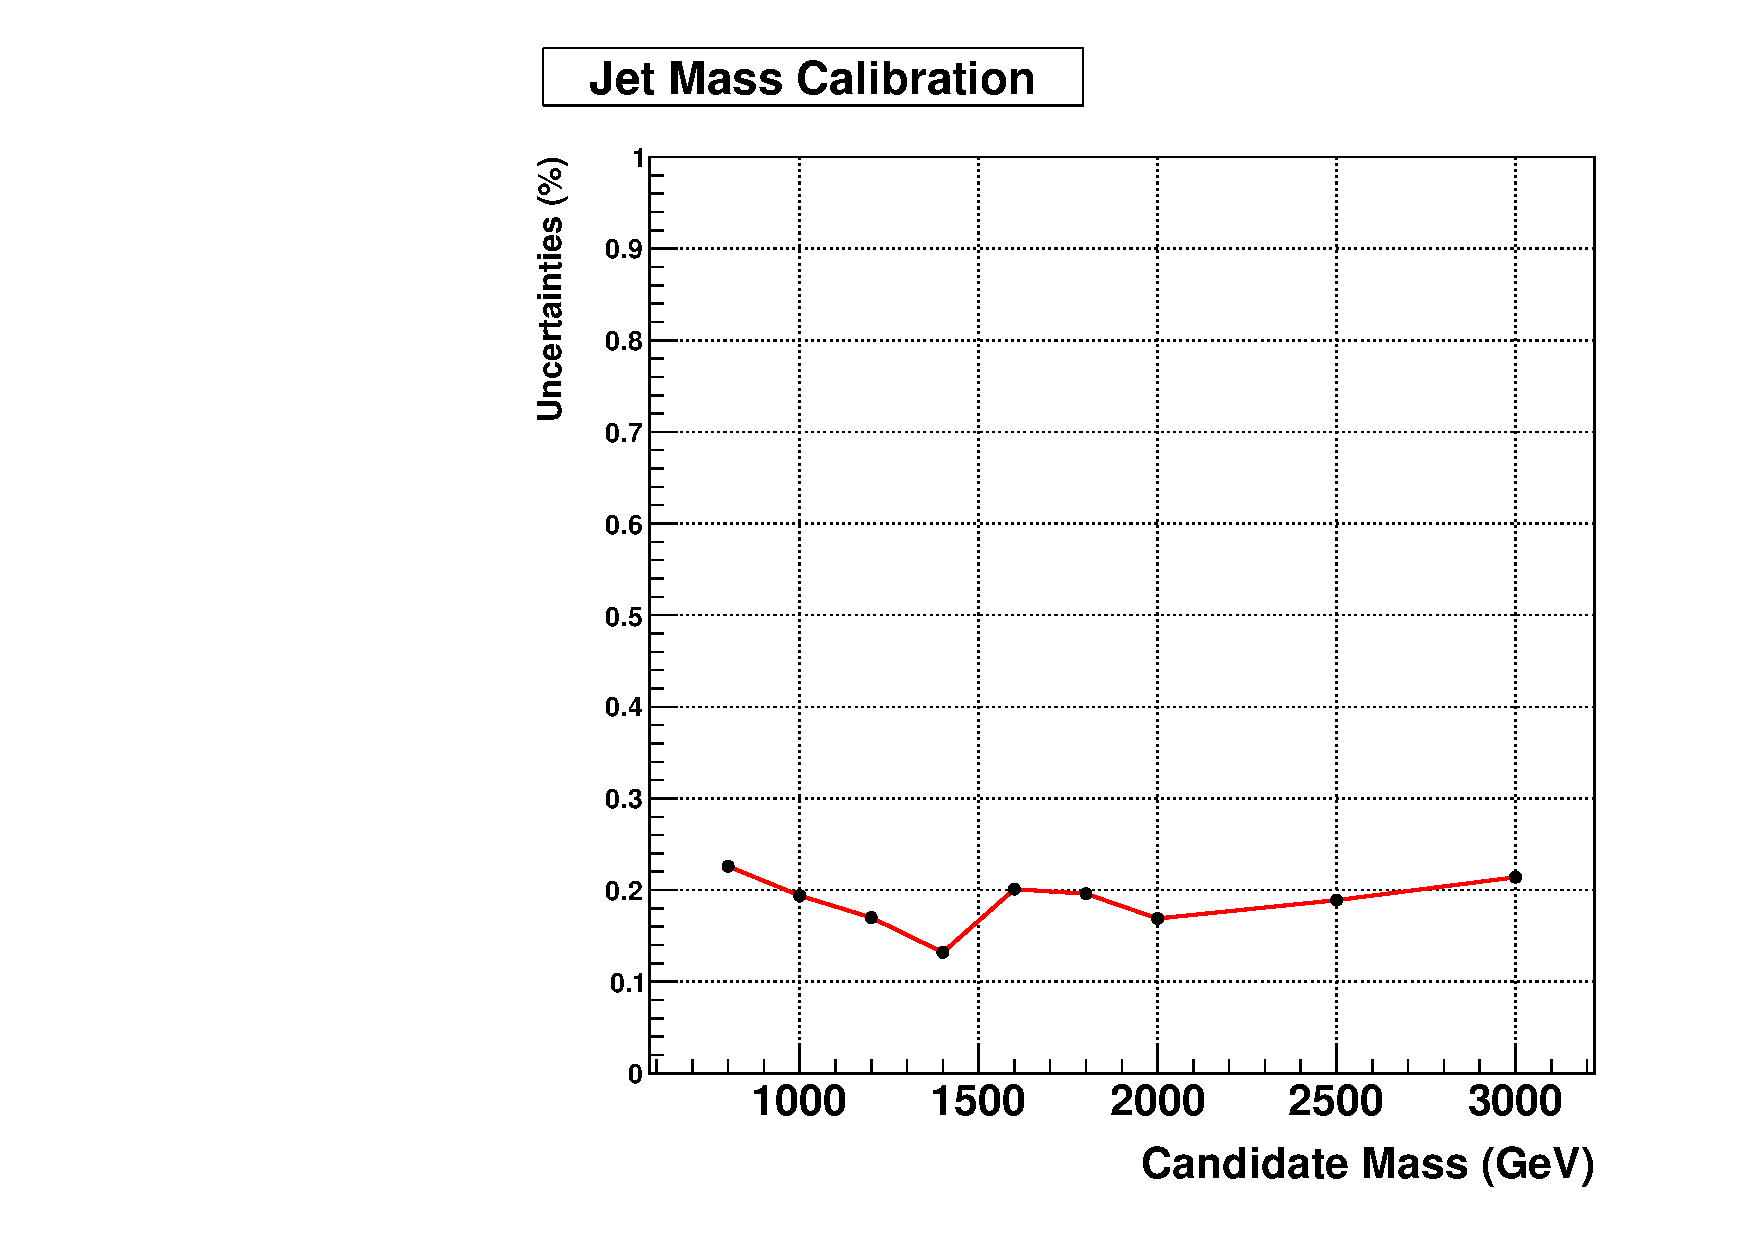
\includegraphics[width=220pt]{figures/SystUncert/JetMassCalib.pdf}\\
\end{tabular}
\label{fig:masscalib}
\end{figure}

\section{Jet mass resolution  uncertainty}

We consider the systematic uncertainties due to the pruned jet mass resolution. In that sense we vary the jet mass resolution from the central value  in order to calculate the impact on the signal selection efficiency. This was applied in the context of 76X with v2 JEC (pruned jet mass + N-subjettiness). Note that in our case the scale factor is one. The shift of the signal peak varies between 0.93$\%$ and 1.50$\%$. The figure \ref{fig:massres} show the systematic uncertainties due to the jet mass resolution for different mass points. 

\begin{figure}[!ht]
\caption{ Systematic uncertainties due to jet mass resolution. The figure shows the systematic uncertainties in $(\%)$ for different mass points.}
\begin{center}
  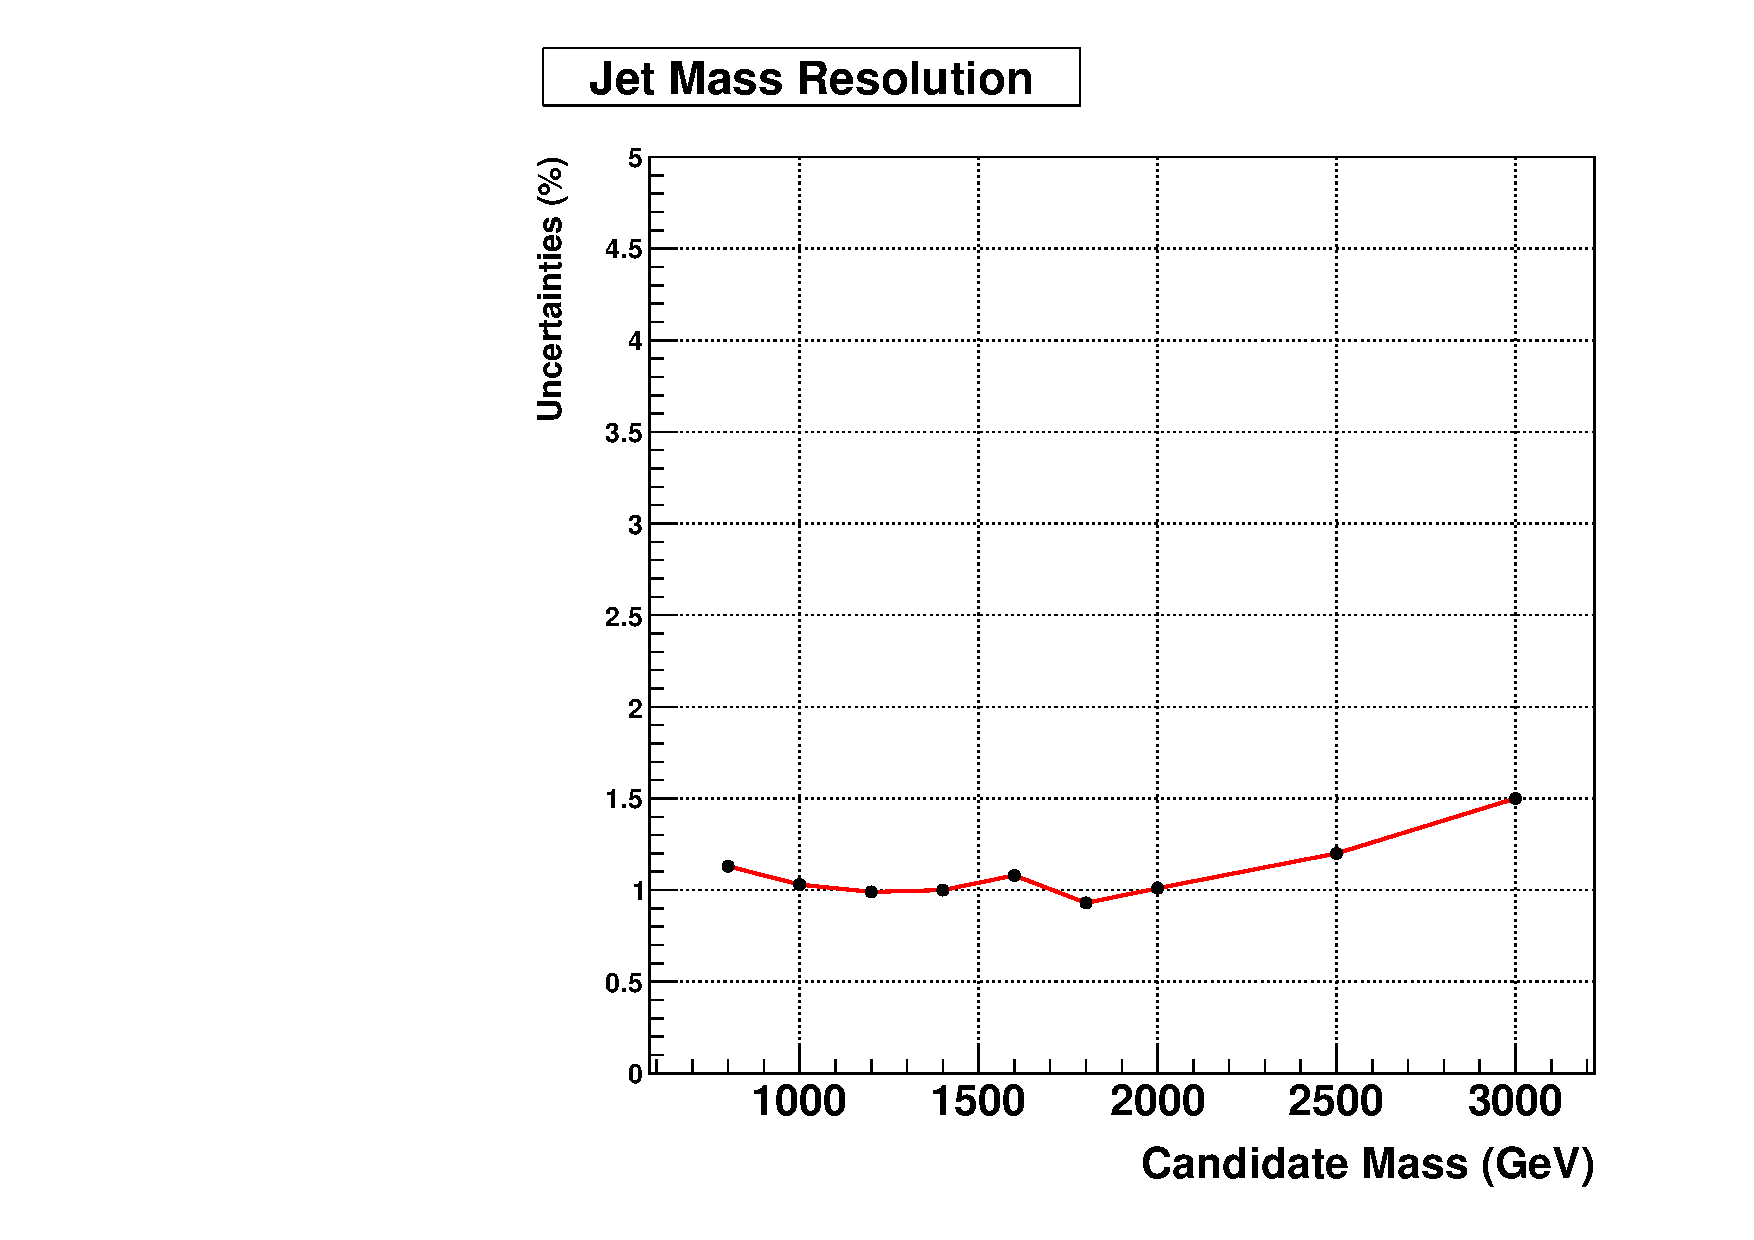
\includegraphics[width=230pt]{figures/SystUncert/JetMassRes.pdf}
\end{center}
\label{fig:massres}
\end{figure}

\section{$\pt$ extrapolation uncertainty}

The impact of the extrapolation uncertainties on the $\tau_{21}$-selection due to propagation to higher momenta is take in account. Extrapolation uncertainties for a W/Z $\pt$ of interest can be estimated from the double ratio of the selection efficiency from Pythia and Herwig samples with W/Z  $\pt$ of 200 GeV and signal with W/Z $\pt$ of interest. We the use the formula : $0.059*\ln(\pt/200)$GeV to estimate this uncertainty. As an approximation we will consider the $\pt$ of the jets as half the value of the mass of the resonance.
The figure \ref{fig:ptextra} show the systematic uncertainties due to the $\pt$ extrapolation for different mass points.

\begin{figure}[!ht]
\caption{ Systematic uncertainties due to $\pt$ extrapolation. The figure shows the systematic uncertainties in $(\%)$ for different mass points.}
\begin{center}
  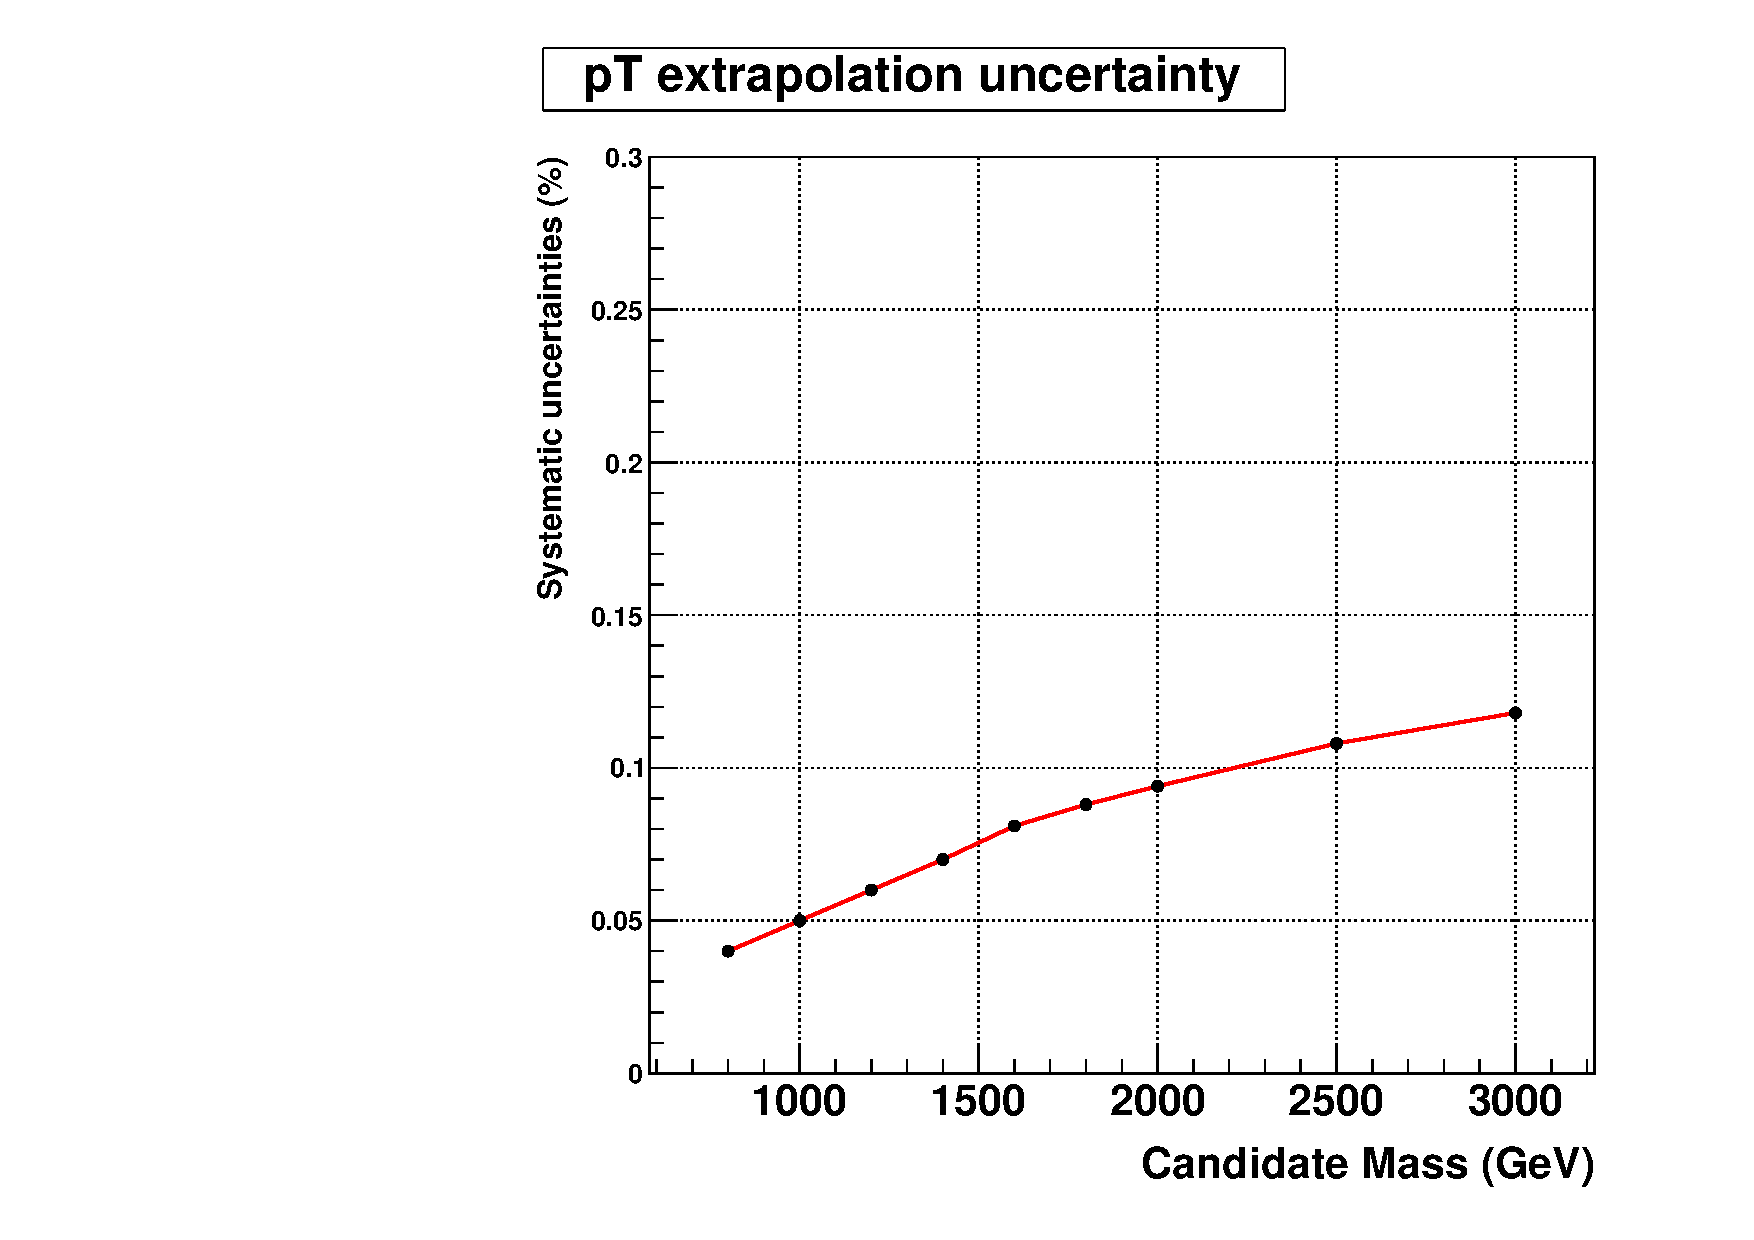
\includegraphics[width=230pt]{figures/SystUncert/ptextra.pdf}
\end{center}
\label{fig:ptextra}
\end{figure}

\section{$\MET$ unclustered energy uncertainty}

We consider the impact of the unclustered enery uncertainties in the analysis. We use the Run2 style varying each particle type by his own resolution. Wit this purpose in 76X we need to rerun the $\MET$ from the miniAOD and use the resolution files provided by the JME POG.  
Then we scale up and down the $\MET$ using the options :
\begin{itemize}
\item
 $\verb|slimmedMET.shiftedPt(pat::MET::UnclusteredEnUp)|$ 
\item
 $\verb|slimmedMET.shiftedPt(pat::MET::UnclusteredEnDown)|$
\end{itemize}
The associated systematic uncertainty due to the shift of the signal peak varies between 0.02$\%$ and 0.13$\%$ for signal and is around 3.6$\%$ for the subdominant backgrounds. \\

\section{Cross section}
Systematics in the normalization of the subdominant backgrounds. of 10$\%$, 20$\%$ and 50$\%$ will be included for the top, di boson and QCD backgrounds respectively to account for the uncertainty in their production cross-sections. 


We summarize the systematic uncertainties obtained in this section in the table \ref{tab:SystUncert}. All the uncertainties with values less equal than  0.5 $\%$ are considering negligibles in the analysis.

\begin{table}[!ht]
\begin{footnotesize}
\centering
\caption{Systematic uncertainties in the analysis.}
\label{tab:SystUncert}
\begin{tabular}{lccc}\hline
 Source  &  Signal  & Dominant  & Subdominant  \\ \hline
 Luminosity &  2.7 $\%$ & - & - \\
 Boosted V-Tagging  & 7$\%$ (HP), 26$\%$ (LP) & - &  7$\%$ (HP), 26$\%$ (LP) \\
 Background estimation & - &  20.5 $\%$ (HP), 15.5$\%$ (LP) & - \\
 Leptons and Photons ID &  0.02 $\%$  & - & -\\
 JEC (Jet and $\MET$) &   0.09-1.76 $\%$  & - & 3$\%$ \\
 JER &   0.009-0.006 $\%$  & - &- \\
 Factorization and renormalization scales &  0.21-0.5 $\%$ & - & 12 $\%$ \\
 PDF &   8-18 $\%$ & - & 17$\%$\\
 Trigger SF & 2.5 $\%$ & - & - \\
 b-tagging efficiency SF &  0.02-0.04$\%$ & 0.05 $\%$  & 1 $\%$  \\
 Pile up &  0.02$\%$  & - & 2.3 $\%$  \\
 Jet mass Calibration & 0.13-0.22 $\%$ & - & - \\
 Jet mass Resolution &  0.93-1.50 $\%$ & - & - \\
 $\pt$ extrapolation uncertainty & 0.04-0.11 $\%$ (HP) & - & - \\
 $\MET$ unclustered energy & 0.02-0.13 $\%$   & -  &  3.6 $\%$ \\
Cross section & -    & -  &  30 $\%$ \\ \hline
\end{tabular}
\end{footnotesize}
\end{table}


\section{Nuisance parameter impacts}

The impact of a nuisance parameter (NP) $\theta$  (systematic uncertanties) on a parameter of interest (POI) $\mu$ (signal strength) is defined as the shift $\Delta \mu$ that is induced as $\theta$ is fixed and brought to its +1$\sigma$ and -1$\sigma$  post-fit values, with all other parameters profiled as normal. This is effectively a measure of the correlation between the NP and the POI, and is useful for determining which NPs have the largest effect on the POI uncertainty. 
The direction of the +1$\sigma$ and -1$\sigma$ impacts on the POI indicates whether the parameter is correlated or anti-correlated with it. Figure \ref{fig:impact} shows the impact of the systematic uncertainties for a bulk graviton signal of 1.2 TeV. 


\begin{figure}[!ht]
\caption{ Impact of the systematic uncertainties in the analysis.}
\begin{center}
  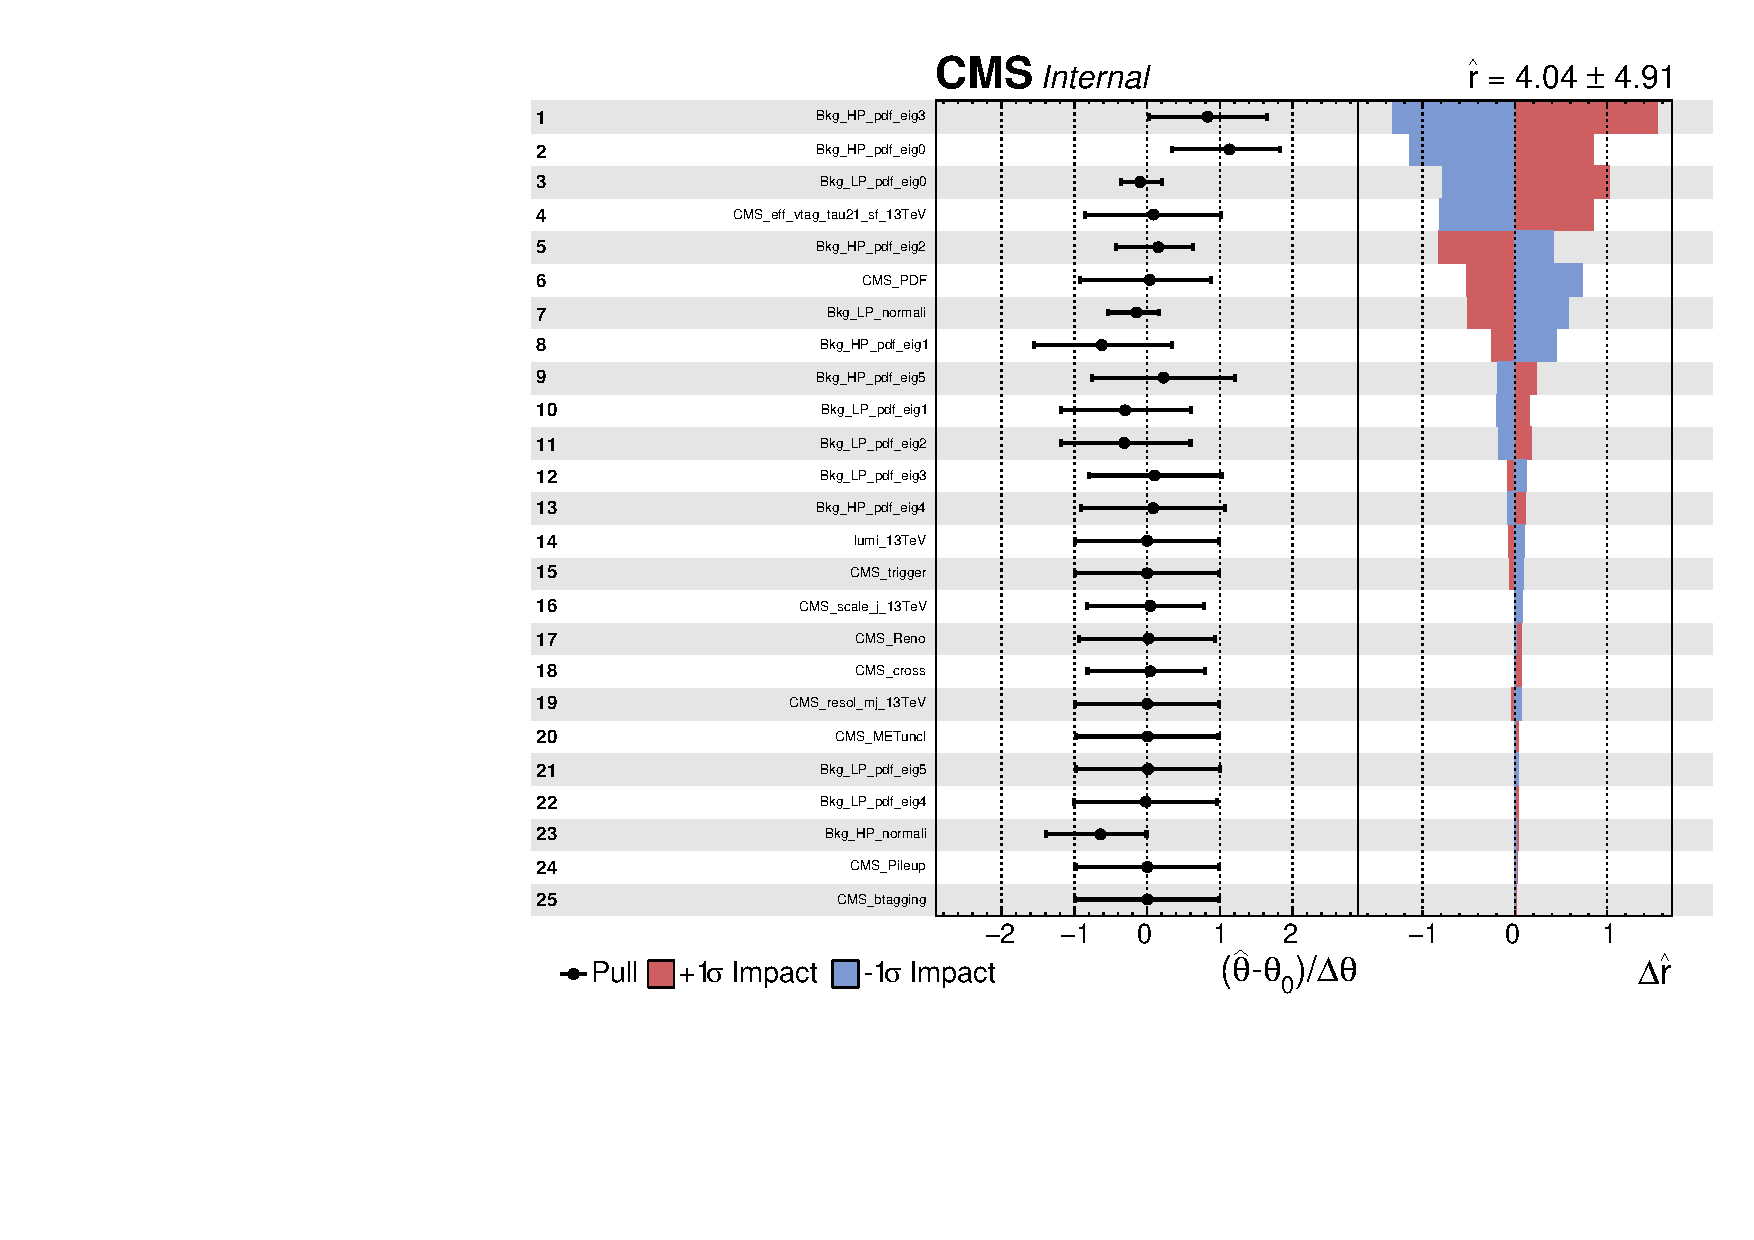
\includegraphics[height=13cm, width=15cm]{figuresARC/systematics/impacts.pdf}
\end{center}
\label{fig:impact}
\end{figure}
